%!TEX root = dissertation.tex
\chapter{State-space deep Gaussian processes}
\label{chap:dssgp}
In this chapter we introduce state-space deep Gaussian processes (SS-DGPs). The chapter starts with a brief review on Gaussian processes (GPs) and their state-space representations in Sections~\ref{sec:gp} and~\ref{sec:ssgp}, respectively. Subsequently, in Section~\ref{sec:ssdgp} deep Gaussian processes and their state-space representations (i.e., SS-DGPs) are defined. In Section~\ref{sec:deep-matern}, we introduce deep \matern processes which are a subclass of SS-DGPs where each GP element in the SS-DGP hierarchy is conditionally a \matern GP. Section~\ref{sec:ssdgp-reg} represents the SS-DGP regression problems as continuous-discrete filtering and smoothing problems. Finally, Section~\ref{sec:l1-r-dgp} illustrates how to solve $L^1$-regularised SS-DGP regression problems.

The content of this chapter is based on Publications~\cp{paperSSDGP} and~\cp{paperRNSSGP}. 

\section{Gaussian processes}
\label{sec:gp}
Gaussian processes (GPs) are a class of stochastic processes with finite-dimensional Gaussian distributions. More precisely, an $\R^d$-valued stochastic process $U\colon\T\to\R^d$ is said to be a GP if the following definition is satisfied. 
%
\begin{definition}[Gaussian process]
	\label{def:gp}
	A stochastic process $U\colon \T\to \R^d$ on some probability space is called a Gaussian process on $\T$ if for every integer $k\geq 0$ and real numbers $t_1<t_2<\cdots<t_k \in \T$, the random variables $U(t_1), U(t_2), \ldots, U(t_k)$ are jointly Gaussian~\citep[see, e.g.,][Section 2.9]{Karatzas1991}. 
\end{definition}
%
\begin{remark}
In the spirit of this thesis, we restrict Definition~\ref{def:gp} to temporal GPs only, however, it is possible to define GPs on more general domains~\citep{Carl2006GPML}.
\end{remark}

Since multivariate normal distributions are entirely determined by their means and covariances, Definition~\ref{def:gp} is usually interpreted by the shorthand notation
%
\begin{equation}
	U(t) \sim \GP\big(m(t), C(t, t')\big),
	\label{equ:gp-notation}
\end{equation}
%
where $m \colon \T \to\R^d$ and $C\colon \T \times \T \to\R^{d \times d}$ stand for the mean and covariance functions of the process, respectively. Under this notation, the finite-dimensional probability density function of $U$ at time instances $t_1, t_2,\ldots, t_k\in\T$ is given by
%
\begin{equation}
	\begin{split}
		&p_{U(t_1), U(t_2), \ldots, U(t_k)}(u_1, u_2, \ldots, u_k) \\
		&= \mathrm{N} 
		\begin{pmatrix}
			\begin{bmatrix}
				u_1 \\ u_2 \\ \vdots \\ u_k
			\end{bmatrix} \condBigg
			\begin{bmatrix}
				m(t_1) \\ m(t_2) \\ \vdots \\ m(t_k)
			\end{bmatrix}, 
			\begin{bmatrix}
				C(t_1, t_1) & C(t_1, t_2) & \cdots & C(t_1, t_k) \\
				C(t_2, t_1) & C(t_2, t_2) & \cdots & C(t_2, t_k) \\
				\vdots & \vdots & \ddots & \vdots \\
				C(t_k, t_1) & C(t_k, t_2) & \cdots & C(t_k, t_k)
			\end{bmatrix}
		\end{pmatrix}.
	\end{split}
\end{equation}
%
There are numerous possible choices for the covariance function $C$, and researchers and practitioners can choose one or the other depending on their applications. One of the most popular family of covariance functions to model continuous functions with varying degrees of regularity is given by the Whittle--Mat\'{e}rn covariance function~\citep{Matern1960}
%
\begin{equation}
	C_{\mathrm{Mat.}}(t, t') = \frac{\sigma^2 \, 2^{1-\nu}}{\varGamma(\nu)} \, \Bigg(\frac{\sqrt{2 \, \nu} \, \abs{t - t'}}{\ell}\Bigg)^\nu \, \mBesselsec \Biggl(\frac{\sqrt{2 \, \nu} \, \abs{t - t'}}{\ell}\Biggr),
	\label{equ:cov-matern}
\end{equation}
%
where $\ell$ and $\sigma$ are scale parameters, $\varGamma$ is the Gamma function, $\mBesselsec$ is the modified Bessel function of the second kind, and $\nu \in \big\lbrace \frac{1}{2}, \frac{3}{2}, \ldots \big\rbrace$. The smoothness of $U$ is controlled by the value of $\nu$. For example, if $\nu = \frac{3}{2}$, then $t\mapsto U(t)$ will be differentiable almost surely.  

Without loss of generality, we assume from now on that $m(t) = 0$ for all $t\in\T$, that is
%
\begin{equation}
	U(t) \sim \GP\big(0, C(t, t')\big).
\end{equation}
%
The covariance function $C$ thus entirely determines the properties of $U$, such as its continuity and stationarity. 
%
\begin{remark}
	\label{remark:stationary-gp}
	A stochastic process $U$ is said to be stationary if its finite-dimensional distribution is invariant under translation. That is,
	\begin{equation}
	p_{U(t_1+\tau),\ldots,U(t_k+\tau)}(u_1, \ldots, u_k) = p_{U(t_1),\ldots,U(t_k)}(u_1, \ldots, u_k), \nonumber
	\end{equation} 
	for all $k\geq 1$, $t_1<\cdots<t_k \in \T$, and $t_1+\tau<\cdots<t_k+\tau \in \T$~\citep{Karatzas1991}. Since GPs are characterised by their mean and covariance functions, we say that a zero-mean GP is stationary if $C(t+\tau, t'+\tau)$ does not depend on $\tau$, or equivalently, $C(t, t')$ is only a function of the time difference $t-t'$. 
\end{remark}
%
Stationarity is an important concept to keep in mind as many widely used covariance functions, such as the Mat\'{e}rn family and the radial basis function (RBF) lead to stationary GPs. However, as mentioned in Introduction, these stationary GPs might not be suitable priors in a number of applications.
%

\subsection*{Batch GP regression}
\label{sec:gp-reg-batch}
Consider a GP regression model
%
\begin{equation}
	\begin{split}
		U(t) &\sim \GP\big(0, C(t, t')\big), \\
		Y_k &= U(t_k) + \xi_k, \quad \xi_k \sim\mathrm{N}(0, \Xi_k),
	\end{split}
	\label{equ:batch-gp-reg}
\end{equation}
%
where we have a set of measurement data $y_{1:T} = \lbrace y_k \colon k=1,2,\ldots, T\rbrace$ at times $t_1, t_2, \ldots, t_T\in\T$. Let us denote by $C_{1:T}$ the (Gram) matrix obtained by evaluating the covariance function $C$ on the Cartesian grid $(t_1, t_2, \ldots, t_T) \times (t_1, t_2, \ldots, t_T)$. Let us also define $\Xi_{1:T} \coloneqq \diag{\Xi_1, \Xi_2, \ldots, \Xi_T}$ and $U_{1:T} \coloneqq \big\lbrace U(t_1), \allowbreak U(t_2), \ldots, U(t_T) \big\rbrace$.

Using Bayes' rule, and Gaussian identities, one can prove that the joint batch posterior probability density $p_{U_{1:T} \cond Y_{1:T}}(u_{1:T} \cond y_{1:T})$ is Gaussian. More specifically, the mean and covariance of the batch posterior density are given by
%
\begin{equation}
	\expec{U_{1:T} \cond y_{1:T}} = C_{1:T} \, (C_{1:T} + \Xi_{1:T})^{-1} \, y_{1:T}
	\label{equ:gp-reg-m}
\end{equation}
%
and
\begin{equation}
	\cov{U_{1:T} \cond y_{1:T}} = C_{1:T} - C_{1:T}\,(C_{1:T} + \Xi_{1:T})^{-1} \, C_{1:T},
	\label{equ:gp-reg-P}
\end{equation}
respectively. With a slight modification of the two equations above, the mean and covariance of the posterior density at test points (i.e., interpolation/extrapolation) can also be obtained in closed-form~\citep[see, e.g.,][Section 2.2]{Carl2006GPML}.
%
\begin{remark}
	The batch term in the name comes from the fact that the posterior density is solved jointly at $t_1, t_2, \ldots, t_T$ by using the full covariance matrix $C_{1:T}$.
\end{remark}
%
In Figure~\ref{fig:gp-fail}, we illustrate two examples of this batch GP regression using a \matern $\nu=3\,/\,2$ covariance function of the form in Equation~\eqref{equ:cov-matern}. 

It is worth pointing out two numerical problems of batch GP regressions. First, the computational complexity for computing the posterior mean and covariance is $O(T^3)$. This is due to the necessity of solving a system of equations of size $T$. This makes standard GP regression computationally expensive for large-scale datasets. This prompted researchers to introduce a number of alternatives (e.g., sparse GPs) that alleviate this prohibitive complexity. We refer the reader to Section~\ref{sec:literature-review} for a short review on this topic.

Another problem is that if the data times $t_1,t_2,\ldots, t_T$ are densely located (i.e., $t_{k} - t_{k-1}$ is numerically small for $k=1,2,\ldots,T$), or when some of them are identical, then the covariance matrix $C_{1:T}$ might be numerically close to singular~\citep[see, e.g.,][]{Ababou1994, Ranjan2011}. This numerical problem does not in general affect the numerical computation of Equations~\eqref{equ:gp-reg-m} and~\eqref{equ:gp-reg-P}, as the minimum eigenvalue of $C_{1:T} + \Xi_{1:T}$ is greater than the minimum eigenvalue of $\Xi_{1:T}$. However, it affects any procedure that needs to compute the matrix inverse of $C_{1:T}$ (e.g., maximum a posterior estimate of GP regression), or that the GP is observed without measurement noises~\citep{Ranjan2011}. It may also affect making samples from GP by means of Cholesky decomposition of $C_{1:T}$.

State-space representations of GPs, as formulated in the following section, can be used to avoid the two problems above.

\section{State-space Gaussian processes}
\label{sec:ssgp}
In this section, we introduce state-space representations of GPs. Namely, we represent GPs as solutions of linear SDEs. In order to do this, let $U \colon \T \to \R^d$ be the solution of a linear SDE
%
\begin{equation}
	\begin{split}
		\diff U(t) &= A(t) \, U(t) \diff t + B(t) \diff W(t), \\
		U(t_0) &= U_0,
	\end{split}
	\label{equ:ssgp}
\end{equation}
%
where coefficients $A \colon \T \to \R^{d \times d}$ and $B \colon \T \to \R^{d \times w}$ are deterministic time-dependent functions, $W\colon\T\to\R^w$ is a Wiener process, and ${U}_0 \sim \mathrm{N}(m_0, P_0)$. For the sake of simplicity, let us from now on assume that these coefficients are regular enough so that the SDE above is well-defined (see, e.g., Theorem~\ref{thm:linear-sde-solution} for sufficient conditions).

It turns out that the solution $U$ of the SDE in Equation~\eqref{equ:ssgp} verifies the axioms of Gaussian processes (given in Definition~\ref{def:gp}) on $\T$~\citep[see,][Section 5.6]{Karatzas1991}. Moreover, its mean $t\mapsto \expec{U(t)}$ and covariance $t\mapsto\cov{U(t)}$ functions are solutions of the following linear ODEs
%
\begin{equation}
	\begin{split}
		\frac{\diff m(t)}{\diff t} &= A(t) \, m(t), \\
		\frac{\diff P(t)}{\diff t} &= A(t) \, P(t) + P(t) \, A(t)^\trans + B(t) \, B(t)^\trans,
	\end{split}
\end{equation}
%
for every $t\in\T$ starting from the initial values $m(t_0) = m_0$ and $P(t_0) = P_0$. Note that if the initial mean $m_0 = 0$ then $m(t) = 0$ for all $t\in\T$, so that $U$ will be a zero-mean GP.

Compared to the batch GP representation in Equation~\eqref{equ:gp-notation}, state-space representations do not need to explicitly specify their mean and covariance functions. These functions are instead implicitly defined by the SDE coefficients. Finding the state-space representation of a GP with desired covariance function is possible as well~\citep[see, e.g.,][]{Hartikainen2010, Simo2013SSGP, Solin2016}.

Suppose that the coefficients $A(t) = A$ and $B(t) = B$ are constants, and all the real parts of the eigenvalues of $A$ are negative. Let $m_0=0$, and let $P_0$ solve the Lyapunov equation
%
\begin{equation}
	A \, P + P \, A^\trans + B \, B^\trans = 0,
	\label{equ:lyapunuv}
\end{equation}
%
then 
\begin{equation}
	U(t) \sim \mathrm{GP}\big(0, \cov{{U}(t), {U}(t')}\big)\nonumber
\end{equation} 
is a zero-mean stationary GP, and its covariance function is given by
%
\begin{equation}
	\cov{{U}(t), {U}(t')} = 
	\begin{cases}
		P_0 \, \expp^{\abs{t-t'} \, A^\trans}, & t < t' \in \T, \\
		\expp^{\abs{t-t'} \, A} \, P_0, & t' \leq t \in \T.
	\end{cases} \nonumber
\end{equation}
See, for example, \citet[][Theorem 6.7]{Karatzas1991}, \citet[][Section 3.7]{Pavliotis2014}, or~\citet[][Section 6.5]{Sarkka2019} for details.

\subsection*{State-space GP regression}
Due to the fact that state-space GPs (SS-GPs) are solutions of SDEs, they verify the Markov property. This is key in allowing to perform GP regression sequentially for $k=1,2,\ldots,T$ without computing the full covariance matrix $C_{1:T}$. To see this, let us consider a GP regression problem in the state-space form
%
\begin{equation}
	\begin{split}
		\diff {U}(t) &= A(t) \, {U}(t) \diff t + B(t) \diff W(t), \quad U(t_0) = U_0,\\
		Y_k &= H_k \, {U}(t_k) + \xi_k, \quad \xi_k \sim \mathrm{N}(0, \Xi_k).
	\end{split}
\end{equation}
%
We aim to compute the posterior density $p_{{U}(t_k) \cond Y_{1:T}}({u}_k \cond y_{1:T})$ for $k=1,2,\ldots, T$ instead of the joint posterior density $p_{U_{1:T} \cond Y_{1:T}}(u_{1:T} \cond y_{1:T})$. This state-space GP regression problem is equivalent to the continuous-discrete smoothing problem in Section~\ref{sec:rts}~\citep{Sarkka2019}. Therefore, one can apply Kalman filters and RTS smoothers (see, Algorithm~\ref{alg:kfs}) to carry out the state-space GP regression at hand exactly. Figure~\ref{fig:gp-kfs-eq} illustrates an example showing the equivalence between batch and state-space GP regression on a toy model. 

The computational complexity of state-space GP regression is $O(T)$, whereas the batch GP regression is $O(T^3)$. As an example, the batch and state-space GP regression shown in Figure~\ref{fig:gp-kfs-eq} take around $37$~s and $0.1$~s, respectively, on a computer with $T=10,000$ measurements.  Furthermore, by using prefix-sum algorithms, state-space GP regression can be solved in logarithmic $O(\log(T))$ time~\citep{Corenflos2021SSGP, Simo2021Parallel}. 

\begin{figure}[t!]
	\centering
	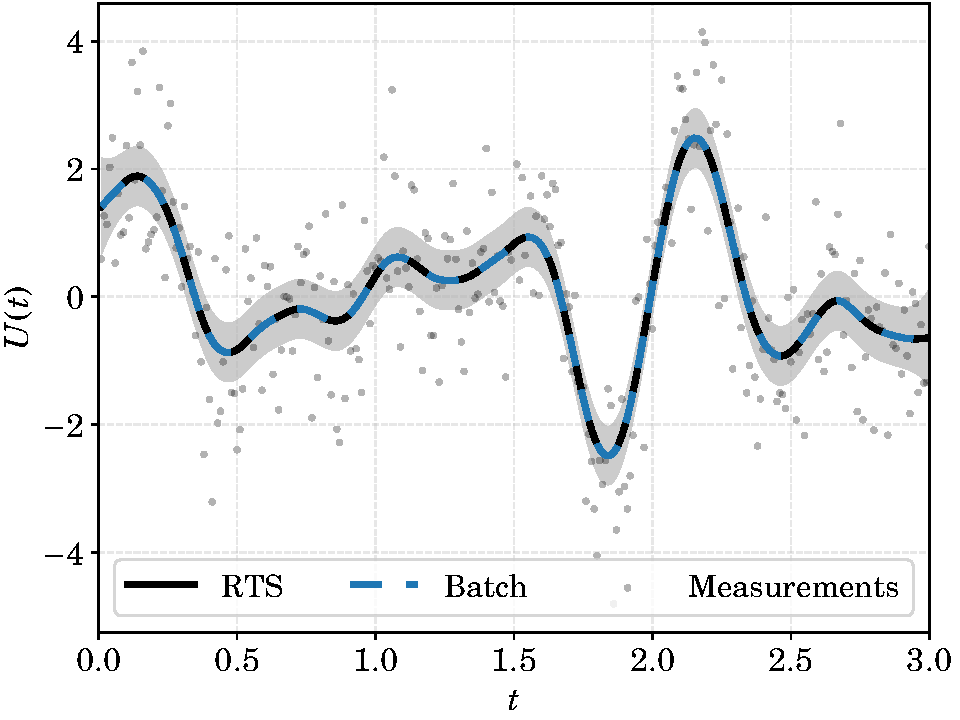
\includegraphics[width=.75\linewidth]{figs/gp-kfs-eq}
	\caption{Batch and state-space GP regression on a toymodel with a \matern $\nu=3\, / \, 2$ covariance function and zero mean function. These two regression methods recover the same posterior densities (the lines and shaded area stand for the posterior mean and 0.95 confidence interval, respectively). }
	\label{fig:gp-kfs-eq}
\end{figure}

It is worth mentioning that not all GPs are Markov processes, hence, not all GPs have analytical state-space representations. As an example, \citet{Rozanov1977, Rozanov1982} show that certain stationary Gaussian processes/fields are Markovian if and only if the reciprocal of their spectral densities are polynomials. For instance, GPs using the RBF covariance function are not Markovian, but it is possible to approximate them up to an arbitrary order by using their approximate state-space representations~\citep{Simo2013SSGP}.

\section{State-space deep Gaussian processes (SS-DGPs)}
\label{sec:ssdgp}
State-space deep Gaussian processes (SS-DGPs) are stochastic processes that parametrise multiple conditional GPs hierarchically. This hierarchical construction makes SS-DGPs suitable priors for modelling irregular function in many applications. To see this, let us first consider a GP
%
\begin{equation}
	U(t) \sim \mathrm{GP}\big(0, C(t, t'; \ell(t)) \big),\nonumber
\end{equation}
%
where the covariance function $C(t, t';\ell(t))$ has an unknown (random) parameter $\ell(t)\in\R_{>0}$ (i.e., a time-varying length scale). When the parameter $\ell(t)$ does not depend on $t$, it can be assigned by human experts or automatically learnt from data by, for example, maximum likelihood estimation (MLE), maximum a posteriori (MAP), variational inference, or Markov chain Monte Carlo (MCMC)~\citep{Carl2006GPML}. However, the assumption that $\ell$ being independent of $t$ might not be reasonable for a number of applications that exhibit time-varying features. A way to mitigate this issue is, for example, to consider putting another GP prior on the length scale parameter, that is
%
\begin{equation}
	\ell(t) \sim \mathrm{GP}\big(0, C(t, t'; \ell_2) \big),\nonumber
\end{equation}
%
where $\ell_2$ is another length scale parameter. This hierarchical feature is meaningful in the sense that it allows the characteristics of $U$ to change over time, since its length scale $t \mapsto \ell(t)$ now is a stochastic process of $t$. It is then of interest to ask if this hierarchical recursion can be continued up to a given depth $L$:
%
\begin{equation}
	\begin{split}
		\ell_2(t) &\sim \mathrm{GP}\big(0, C(t, t'; \ell_3(t)) \big), \\
		\ell_3(t) &\sim \mathrm{GP}\big(0, C(t, t'; \ell_4(t)) \big), \\
		&\vdots\\
		\ell_{L}(t) &\sim \mathrm{GP}\big(0, C(t, t'; \ell_{L+1}) \big),
		\label{equ:cascading-ell}
	\end{split}
\end{equation}
where the final leaf $\ell_{L+1}$ is a constant.
%
This construction leads to a class of deep Gaussian processes (DGPs, see, Section~\ref{sec:literature-review} for background). 

In the rest of this chapter, we formulate the hierarchy in Equation~\eqref{equ:cascading-ell} in more abstract form in order to define DGPs. Thereupon we leverage this definition to represent DGPs as solutions of SDEs in order to arrive at SS-DGPs.

\subsection*{Deep Gaussian processes}
\label{sec:dgp-motiv-def}
Equation~\eqref{equ:cascading-ell} exemplifies a DGP where the length scale parameters \textit{only} are considered as GPs. In graph theory, this type of DGP hierarchy corresponds to a path graph~\citep{Gross2019} where the length scale parameters are vertices that ordered in a line/path. This type of DGP construction is the most studied case in the parametrisation-based DGP community~\citep{Roininen2016, Salimbeni2017ns, Emzir2020}. 

However, in principle, a GP can take any number of parameters. Thus, in order to abstract DGPs, we need to think of a DGP as a joint process defined over a set of conditional GPs. These conditional GPs are not necessarily limited to representing length scale parameters only. In order to do so, we need to introduce an indexing system and a few notations. Let $U^i_j \colon \T \to \R^{d_i}$ denote a GP indexed by an integer $i\in\N$. This superscript $i$ means that $U^i_j$ is the $i$-th GP element in a (yet to be defined) collection of GPs. The subscript $j$ in $U^i_j$ means that the GP $U^i_j$ is a parent of the $j$-th GP element (i.e., the $j$-th GP element is parametrised by the $i$-th element). The terminology ``parent'' follows from probabilistic graph model conventions~\citep{Koller2009}. The fact that GP element does not have any child means that it does not parametrise any other GP therefore, we define its subscript $j$ to be $j=0$. This is always true for the first element $U^1_0$ as we shall see later in the definition of the collection of these GP elements. 

Additionally, in order to give a well-defined graph, we restrict $j<i$ so that a GP element can only parametrise \emph{one} of its \emph{preceding} elements. This implies that a GP element can have multiple parents but no more than one child. Without this restriction, one might have two elements, for instance, $U^2_1$ and $U^1_2$ depending on each other, that is not within the scope of this thesis.
\begin{remark}
	The set of dependencies between the conditional GPs can be thought of as a collection of directed trees where the head of each tree has $j$ subscript $j=0$, and the notation $U_j^i$ implies that there is an edge pointing from $U_j^i$ to $U^j_k$ for some $k$. See, Figure~\ref{fig:dgp-examples-graph} for an illustration.
\end{remark}

Suppose that we have $L$ GPs $U^1_0, U^2_{j_2},\ldots, U^L_{j_L}$ and a set $J = \lbrace j_i \in \N \colon i=1,2\ldots,L, \, \, 0\leq j_i < i\rbrace$ that describes the conditional dependencies of these GPs. We define the collection of all these GPs as
%
\begin{equation}
	\mathcal{V} \coloneqq \mathcal{V}^L_J = \big\lbrace U^i_{j_i} \colon i= 1,2,\ldots, L, \,\, j_i \in J \big\rbrace,
	\label{equ:dgp-set-V}
\end{equation}
%
and we will call these conditional GPs the GP elements of $\mathcal{V}$. Based on this collection, we define a DGP as a vector-valued process composed of all the GP elements in $\mathcal{V}$.

\begin{definition}[Deep Gaussian process]
	\label{def:dgp}
	Let $\mathcal{V}$ be a collection of $L$ $\R^{d_i}$-valued conditional GPs defined by Equation~\eqref{equ:dgp-set-V}. An $\R^{\sum^L_{i=1} d_i}$-valued stochastic process $V \colon \T \to \R^{\sum^L_{i=1} d_i}$ is said to be a deep Gaussian process on $\T$ with respect to $\mathcal{V}$ if $V$ is a permutation of all the elements of $\mathcal{V}$.
\end{definition}

\begin{remark}
	Note that in the special case $L=1$, a DGP reduces to a standard GP. 
\end{remark}

\begin{figure}[t!]
	\centering
	\resizebox{.42\linewidth}{!}{%
		\tikzset{every picture/.style={line width=0.75pt}} %set default line width to 0.75pt        

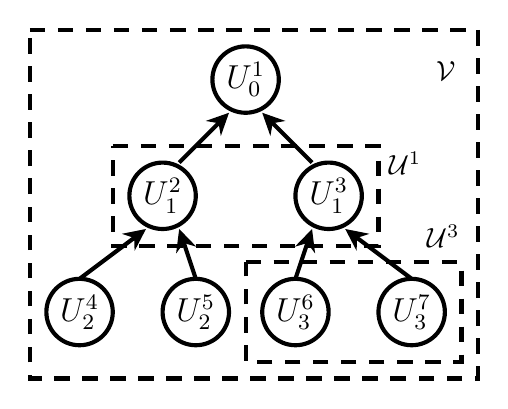
\begin{tikzpicture}[x=0.6pt,y=0.6pt,yscale=-1,xscale=1]
%uncomment if require: \path (0,300); %set diagram left start at 0, and has height of 300

%Shape: Circle [id:dp821654118938725] 
\draw  [line width=1.5]  (200,30) .. controls (200,18.95) and (208.95,10) .. (220,10) .. controls (231.05,10) and (240,18.95) .. (240,30) .. controls (240,41.05) and (231.05,50) .. (220,50) .. controls (208.95,50) and (200,41.05) .. (200,30) -- cycle ;
%Shape: Circle [id:dp7532382575897598] 
\draw  [line width=1.5]  (150,100) .. controls (150,88.95) and (158.95,80) .. (170,80) .. controls (181.05,80) and (190,88.95) .. (190,100) .. controls (190,111.05) and (181.05,120) .. (170,120) .. controls (158.95,120) and (150,111.05) .. (150,100) -- cycle ;
%Shape: Circle [id:dp5902978501813476] 
\draw  [line width=1.5]  (250,100) .. controls (250,88.95) and (258.95,80) .. (270,80) .. controls (281.05,80) and (290,88.95) .. (290,100) .. controls (290,111.05) and (281.05,120) .. (270,120) .. controls (258.95,120) and (250,111.05) .. (250,100) -- cycle ;
%Straight Lines [id:da9016881764549007] 
\draw [line width=1.5]    (207.17,52.83) -- (180,80) ;
\draw [shift={(210,50)}, rotate = 135] [fill={rgb, 255:red, 0; green, 0; blue, 0 }  ][line width=0.08]  [draw opacity=0] (13.4,-6.43) -- (0,0) -- (13.4,6.44) -- (8.9,0) -- cycle    ;
%Straight Lines [id:da026586992089503658] 
\draw [line width=1.5]    (232.83,52.83) -- (260,80) ;
\draw [shift={(230,50)}, rotate = 45] [fill={rgb, 255:red, 0; green, 0; blue, 0 }  ][line width=0.08]  [draw opacity=0] (13.4,-6.43) -- (0,0) -- (13.4,6.44) -- (8.9,0) -- cycle    ;
%Shape: Circle [id:dp7932559631044391] 
\draw  [line width=1.5]  (100,170) .. controls (100,158.95) and (108.95,150) .. (120,150) .. controls (131.05,150) and (140,158.95) .. (140,170) .. controls (140,181.05) and (131.05,190) .. (120,190) .. controls (108.95,190) and (100,181.05) .. (100,170) -- cycle ;
%Shape: Circle [id:dp8827895580667542] 
\draw  [line width=1.5]  (170,170) .. controls (170,158.95) and (178.95,150) .. (190,150) .. controls (201.05,150) and (210,158.95) .. (210,170) .. controls (210,181.05) and (201.05,190) .. (190,190) .. controls (178.95,190) and (170,181.05) .. (170,170) -- cycle ;
%Shape: Circle [id:dp1311962702995253] 
\draw  [line width=1.5]  (230,170) .. controls (230,158.95) and (238.95,150) .. (250,150) .. controls (261.05,150) and (270,158.95) .. (270,170) .. controls (270,181.05) and (261.05,190) .. (250,190) .. controls (238.95,190) and (230,181.05) .. (230,170) -- cycle ;
%Shape: Circle [id:dp055039676738894316] 
\draw  [line width=1.5]  (300,170) .. controls (300,158.95) and (308.95,150) .. (320,150) .. controls (331.05,150) and (340,158.95) .. (340,170) .. controls (340,181.05) and (331.05,190) .. (320,190) .. controls (308.95,190) and (300,181.05) .. (300,170) -- cycle ;
%Straight Lines [id:da3720861628053822] 
\draw [line width=1.5]    (156.8,122.4) -- (120,150) ;
\draw [shift={(160,120)}, rotate = 143.13] [fill={rgb, 255:red, 0; green, 0; blue, 0 }  ][line width=0.08]  [draw opacity=0] (13.4,-6.43) -- (0,0) -- (13.4,6.44) -- (8.9,0) -- cycle    ;
%Straight Lines [id:da5765340159287278] 
\draw [line width=1.5]    (181.26,123.79) -- (190,150) ;
\draw [shift={(180,120)}, rotate = 71.57] [fill={rgb, 255:red, 0; green, 0; blue, 0 }  ][line width=0.08]  [draw opacity=0] (13.4,-6.43) -- (0,0) -- (13.4,6.44) -- (8.9,0) -- cycle    ;
%Straight Lines [id:da8546030008258803] 
\draw [line width=1.5]    (258.74,123.79) -- (250,150) ;
\draw [shift={(260,120)}, rotate = 108.43] [fill={rgb, 255:red, 0; green, 0; blue, 0 }  ][line width=0.08]  [draw opacity=0] (13.4,-6.43) -- (0,0) -- (13.4,6.44) -- (8.9,0) -- cycle    ;
%Straight Lines [id:da21589979146129545] 
\draw [line width=1.5]    (283.2,122.4) -- (320,150) ;
\draw [shift={(280,120)}, rotate = 36.87] [fill={rgb, 255:red, 0; green, 0; blue, 0 }  ][line width=0.08]  [draw opacity=0] (13.4,-6.43) -- (0,0) -- (13.4,6.44) -- (8.9,0) -- cycle    ;
%Shape: Rectangle [id:dp24854624791356805] 
\draw  [dash pattern={on 5.63pt off 4.5pt}][line width=1.5]  (140,70) -- (300,70) -- (300,130) -- (140,130) -- cycle ;
%Shape: Rectangle [id:dp15950228071348826] 
\draw  [dash pattern={on 5.63pt off 4.5pt}][line width=1.5]  (220,140) -- (350,140) -- (350,200) -- (220,200) -- cycle ;
%Shape: Rectangle [id:dp8128591939925793] 
\draw  [dash pattern={on 5.63pt off 4.5pt}][line width=1.5]  (90,0) -- (360,0) -- (360,210) -- (90,210) -- cycle ;

% Text Node
\draw (340.5,25) node    {$\mathcal{V}$};
% Text Node
\draw (316,80.5) node    {$\mathcal{U}^{1}$};
% Text Node
\draw (339,124.5) node    {$\mathcal{U}^{3}$};
% Text Node
\draw (220,30) node  [font=\large]  {$U_{0}^{1}$};
% Text Node
\draw (170,100) node  [font=\large]  {$U_{1}^{2}$};
% Text Node
\draw (270,100) node  [font=\large]  {$U_{1}^{3}$};
% Text Node
\draw (120,170) node  [font=\large]  {$U_{2}^{4}$};
% Text Node
\draw (190,170) node  [font=\large]  {$U_{2}^{5}$};
% Text Node
\draw (250,170) node  [font=\large]  {$U_{3}^{6}$};
% Text Node
\draw (320,170) node  [font=\large]  {$U_{3}^{7}$};

\end{tikzpicture}

	}
	\resizebox{.379\linewidth}{!}{%
		\tikzset{every picture/.style={line width=0.75pt}} %set default line width to 0.75pt        

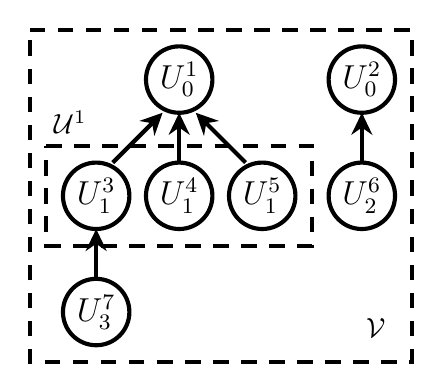
\begin{tikzpicture}[x=0.6pt,y=0.6pt,yscale=-1,xscale=1]
	%uncomment if require: \path (0,300); %set diagram left start at 0, and has height of 300
	
	%Shape: Circle [id:dp821654118938725] 
	\draw  [line width=1.5]  (130,70) .. controls (130,58.95) and (138.95,50) .. (150,50) .. controls (161.05,50) and (170,58.95) .. (170,70) .. controls (170,81.05) and (161.05,90) .. (150,90) .. controls (138.95,90) and (130,81.05) .. (130,70) -- cycle ;
	%Shape: Circle [id:dp7532382575897598] 
	\draw  [line width=1.5]  (80,140) .. controls (80,128.95) and (88.95,120) .. (100,120) .. controls (111.05,120) and (120,128.95) .. (120,140) .. controls (120,151.05) and (111.05,160) .. (100,160) .. controls (88.95,160) and (80,151.05) .. (80,140) -- cycle ;
	%Shape: Circle [id:dp5902978501813476] 
	\draw  [line width=1.5]  (180,140) .. controls (180,128.95) and (188.95,120) .. (200,120) .. controls (211.05,120) and (220,128.95) .. (220,140) .. controls (220,151.05) and (211.05,160) .. (200,160) .. controls (188.95,160) and (180,151.05) .. (180,140) -- cycle ;
	%Straight Lines [id:da9016881764549007] 
	\draw [line width=1.5]    (137.17,92.83) -- (110,120) ;
	\draw [shift={(140,90)}, rotate = 135] [fill={rgb, 255:red, 0; green, 0; blue, 0 }  ][line width=0.08]  [draw opacity=0] (13.4,-6.43) -- (0,0) -- (13.4,6.44) -- (8.9,0) -- cycle    ;
	%Straight Lines [id:da026586992089503658] 
	\draw [line width=1.5]    (162.83,92.83) -- (190,120) ;
	\draw [shift={(160,90)}, rotate = 45] [fill={rgb, 255:red, 0; green, 0; blue, 0 }  ][line width=0.08]  [draw opacity=0] (13.4,-6.43) -- (0,0) -- (13.4,6.44) -- (8.9,0) -- cycle    ;
	%Straight Lines [id:da8305170432215097] 
	\draw [line width=1.5]    (150,94) -- (150,120) ;
	\draw [shift={(150,90)}, rotate = 90] [fill={rgb, 255:red, 0; green, 0; blue, 0 }  ][line width=0.08]  [draw opacity=0] (13.4,-6.43) -- (0,0) -- (13.4,6.44) -- (8.9,0) -- cycle    ;
	%Shape: Circle [id:dp5384623722514443] 
	\draw  [line width=1.5]  (130,140) .. controls (130,128.95) and (138.95,120) .. (150,120) .. controls (161.05,120) and (170,128.95) .. (170,140) .. controls (170,151.05) and (161.05,160) .. (150,160) .. controls (138.95,160) and (130,151.05) .. (130,140) -- cycle ;
	%Shape: Circle [id:dp16437012307038867] 
	\draw  [line width=1.5]  (80,210) .. controls (80,198.95) and (88.95,190) .. (100,190) .. controls (111.05,190) and (120,198.95) .. (120,210) .. controls (120,221.05) and (111.05,230) .. (100,230) .. controls (88.95,230) and (80,221.05) .. (80,210) -- cycle ;
	%Shape: Circle [id:dp734554865123197] 
	\draw  [line width=1.5]  (240,70) .. controls (240,58.95) and (248.95,50) .. (260,50) .. controls (271.05,50) and (280,58.95) .. (280,70) .. controls (280,81.05) and (271.05,90) .. (260,90) .. controls (248.95,90) and (240,81.05) .. (240,70) -- cycle ;
	%Shape: Circle [id:dp48143471465976706] 
	\draw  [line width=1.5]  (240,140) .. controls (240,128.95) and (248.95,120) .. (260,120) .. controls (271.05,120) and (280,128.95) .. (280,140) .. controls (280,151.05) and (271.05,160) .. (260,160) .. controls (248.95,160) and (240,151.05) .. (240,140) -- cycle ;
	%Straight Lines [id:da6721182832003427] 
	\draw [line width=1.5]    (100,164) -- (100,171) -- (100,190) ;
	\draw [shift={(100,160)}, rotate = 90] [fill={rgb, 255:red, 0; green, 0; blue, 0 }  ][line width=0.08]  [draw opacity=0] (13.4,-6.43) -- (0,0) -- (13.4,6.44) -- (8.9,0) -- cycle    ;
	%Straight Lines [id:da34999125713295975] 
	\draw [line width=1.5]    (260,94) -- (260,120) ;
	\draw [shift={(260,90)}, rotate = 90] [fill={rgb, 255:red, 0; green, 0; blue, 0 }  ][line width=0.08]  [draw opacity=0] (13.4,-6.43) -- (0,0) -- (13.4,6.44) -- (8.9,0) -- cycle    ;
	%Shape: Rectangle [id:dp18541931062860906] 
	\draw  [dash pattern={on 5.63pt off 4.5pt}][line width=1.5]  (60,40) -- (290,40) -- (290,240) -- (60,240) -- cycle ;
	%Shape: Rectangle [id:dp6446344359743517] 
	\draw  [dash pattern={on 5.63pt off 4.5pt}][line width=1.5]  (70,110) -- (230,110) -- (230,170) -- (70,170) -- cycle ;
	
	% Text Node
	\draw (150,70) node  [font=\large]  {$U_{0}^{1}$};
	% Text Node
	\draw (100,140) node  [font=\large]  {$U_{1}^{3}$};
	% Text Node
	\draw (200,140) node  [font=\large]  {$U_{1}^{5}$};
	% Text Node
	\draw (150,140) node  [font=\large]  {$U_{1}^{4}$};
	% Text Node
	\draw (100,210) node  [font=\large]  {$U_{3}^{7}$};
	% Text Node
	\draw (260,70) node  [font=\large]  {$U_{0}^{2}$};
	% Text Node
	\draw (260,140) node  [font=\large]  {$U_{2}^{6}$};
	% Text Node
	\draw (73,87.4) node [anchor=north west][inner sep=0.75pt]    {$\mathcal{U}^{1}$};
	% Text Node
	\draw (261,212.4) node [anchor=north west][inner sep=0.75pt]    {$\mathcal{V}$};
	
	
\end{tikzpicture}

	}
	\caption{Two DGP ($L=7$) examples in graph illustration.}
	\label{fig:dgp-examples-graph}
\end{figure}

It is also natural to define another set 
%
\begin{equation}
	\mathcal{U}^i = \big\lbrace U^k_{i} \in \mathcal{V} \colon k = 1,2,\ldots, L \big\rbrace
	\label{equ:dgp-set-Ui}
\end{equation}
% 
that collects all the parent GPs of the $i$-th GP element in $\mathcal{V}$. It follows from Lemma~\ref{lemma:dgp-graph-partition} that all the collections of parent GPs form a partition of the set of all GP elements.

\begin{lemma}[Partition]
	\label{lemma:dgp-graph-partition}
	Let $ \mathcal{U}^0, \mathcal{U}^1, \ldots, \mathcal{U}^L$ be collections of parent GPs as defined by Equation~\eqref{equ:dgp-set-Ui}. These collections satisfy the axiom of a partition.
	\begin{enumerate}[I.]
		\item (Pairwise disjointness) For every $m,n\in\lbrace 0, 1,\ldots,L-1\rbrace$ and $m\neq n$,
		\begin{equation}
			\mathcal{U}^m \cap \mathcal{U}^n = \emptyset.
		\end{equation}
		\item (Exhaustiveness)
		\begin{equation}
			\bigcup_{i=0}^{L-1} \mathcal{U}^i = \mathcal{V}.
	\end{equation}
	\end{enumerate}
\end{lemma}
\begin{remark}
	Note that $\mathcal{U}^L=\emptyset$ by construction.
\end{remark}
\begin{proof}
	In order to prove the first property, suppose that there exists a pair $m,n\in\lbrace 0, 1,\ldots,L-1\rbrace$ and $m\neq n$ such that $\mathcal{U}^m \cap \mathcal{U}^n$ is non-empty. This implies that there is a GP element pointing simultaneously to $U^m_{j_m}$ and to $U^n_{j_n}$, which violates the definition of a GP element. 

	Following Equations~\eqref{equ:dgp-set-V} and~\eqref{equ:dgp-set-Ui}, we have $\bigcup^{L-1}_{i=0} \mathcal{U}^i \subseteq \mathcal{V}$. Suppose that there exists a GP element that is in $\mathcal{V}$ but not in $\bigcup^{L-1}_{i=0} \mathcal{U}^i$, then this GP element is not a parent of any GP elements (i.e., it must be in $\mathcal{U}^0$) which violates the hypothesis.
\end{proof}

We mention that the indexing system for DGPs here is simplified compared to Publication~\cp{paperSSDGP} which additionally used an unnecessary index denoting the depth of the GP element in the hierarchy. Figure~\ref{fig:dgp-examples-graph} illustrates two graphical examples of DGPs to clarify the indexing and notations used here. 

\subsection*{Batch representations of DGPs}
\label{sec:batch-ss-dgps}
Following Definition~\ref{def:dgp}, we can use the following shorthand batch notation to represent a DGP $V\colon \T\to\R^{\sum^L_{i=1} d_i}$ with $L$ conditional GPs: 

\begin{equation}
	\begin{split}
		U^1_0(t) \condbig \mathcal{U}^1 &\sim \mathrm{GP}\big(0, C^1(t, t'; \mathcal{U}^1)\big), \\
		U^2_{j_2}(t) \condbig \mathcal{U}^2 &\sim \mathrm{GP}\big(0, C^2(t, t'; \mathcal{U}^2)\big), \\
		&\vdots\\
		U^i_{j_i}(t) \condbig \mathcal{U}^i &\sim \mathrm{GP}\big(0, C^i(t, t'; \mathcal{U}^i)\big), \\
		&\vdots\\
		U^L_{j_L}(t) &\sim \mathrm{GP}\big(0, C^L(t, t')\big),
		\label{equ:batch-dgp}
	\end{split}
\end{equation}
where $C^i\colon \T \times \T \to \R^{d_i \times d_i}$ is the covariance function of $U^i_{j_i}$ parametrised by the GPs in $\mathcal{U}^i$, and
\begin{equation}
	V(t) \coloneqq \begin{bmatrix} U^1_0(t) & U^2_{j_2}(t) & \cdots & U^L_{j_L}(t) \end{bmatrix}^\trans. \nonumber
\end{equation}
Thanks to the conditional hierarchy structure of the model, the probability density function
%
\begin{equation}
	\begin{split}
		p_{V(t)}(v, t) &\coloneqq p_{U^1_0(t),\ldots,U^L_{j_L}(t)}\big(u^1_0,\ldots,u^L_{j_L}, t\big) \\
		&= \prod^L_{i=1} p_{U^i_{j_i}(t) \cond \mathcal{U}^i} \big(u^i_{j_i}, t \cond \mathcal{U}^i \big)
		\label{equ:batch-dgp-density}
	\end{split}
\end{equation}
%
of $V$ can factorise over the probability densities of the GP elements $p_{U^i_{j_i}(t) \cond \mathcal{U}^i} \allowbreak \big(u^i_{j_i}, t \cond \mathcal{U}^i \big)$ for $i=1,\ldots, L$. Notice that for the sake of readability, we slightly abused the notation in Equation~\eqref{equ:batch-dgp-density}, in the sense that $\mathcal{U}^i$, appearing in the argument of $p_{U^i_{j_i}(t) \cond \mathcal{U}^i} \big(u^i_{j_i}, t \cond \mathcal{U}^i \big)$, actually stands for the realisation of all the GPs contained in $\mathcal{U}^i$. 

In order for the DGP $V$ represented by Equation~\eqref{equ:batch-dgp} to be well-defined, its covariance functions $C^1,\ldots, C^L$ must be chosen suitably. Many conventional covariance functions -- such as the Mat\'{e}rn $C_{\mathrm{Mat.}}$ in Equation~\eqref{equ:cov-matern} -- mostly fail to be positive definite if one replaces their parameters with time dependent functions. To allow for time-varying parameters, a typical choice is to use
%
\begin{equation}
	\begin{split}
		&C_{\mathrm{NS}}(t, t'; \ell, \sigma) \\
		&= \frac{\sigma(t) \, \sigma(t') \big(\ell(t) \, \ell(t')\big)^{\frac{1}{4}} \, \sqrt{2}}{\varGamma(\nu) \, 2^{\nu-1} \, \sqrt{\ell(t) + \ell(t')}} \left(\sqrt{\frac{8 \, \nu \, (t-t')^2}{\ell(t) + \ell(t')}}\right)^{\!\!\nu} \mBesselsec\!\left(\sqrt{\frac{8 \, \nu \, (t-t')^2}{\ell(t) + \ell(t')}}\right),
		\label{equ:cov-ns-matern}
	\end{split}
\end{equation}
%
which is a non-stationary generalisation of the Mat\'{e}rn family by~\citet{Paciorek2004, Paciorek2006}. \citet{Gibbs} introduces a similar formulation for constructing a non-stationary RBF covariance function. More non-stationary covariance function examples using time-varying parameters can also be found in, for example, \citet{Higdon1999non, Snoek2014, Remes2017}.

\subsection*{State-space representations of DGPs}
Another way to represent a DGP as defined in Definition~\ref{def:dgp} is through the use of SDEs. The idea consists in forming a (non-linear) system of SDE representations of all the GP elements appearing in the hierarchy. More precisely, let $U^1_0, U^2_{j_2}, \ldots, U^i_{j_i}, \ldots, U^L_{j_L}$ be $\R^{d_i}$-valued GPs that satisfy the following SDEs
%
\begin{equation}
	\begin{split}
		\diff U^1_0(t) &= A^1\big(t; \mathcal{U}^1\big) \, U^1_0 \diff t + B^1\big(t; \mathcal{U}^1\big) \diff W^1(t), \\
		\diff U^2_{j_2}(t) &= A^2\big(t; \mathcal{U}^2\big) \, U^2_{j_2} \diff t + B^2\big(t; \mathcal{U}^2\big) \diff W^2(t), \\
		&\vdots \\
		\diff U^i_{j_i}(t) &= A^i\big(t; \mathcal{U}^i\big) \, U^i_{j_i} \diff t + B^i\big(t; \mathcal{U}^i\big) \diff W^i(t), \\
		&\vdots \\
		\diff U^L_{j_L}(t) &= A^L(t) \, U^L_{j_L} \diff t + B^L(t) \diff W^L(t),
		\label{equ:ss-dgps-sde-split}
	\end{split}
\end{equation}
%
respectively.
In Equation~\eqref{equ:ss-dgps-sde-split}, $W^i \colon \T \to \R^{w_i}$ for $i=1,2,\ldots, L$ are $w_i$-dimensional Wiener processes, and $A^i \colon \T \to \R^{d_i \times d_i}$ and $B^i \colon \T \to \R^{d_i \times w_i}$ for $i=1,2,\ldots, L-1$ are stochastic processes that are parametrised by the GPs in $\mathcal{U}^i$. The $L$-th coefficients $A^L\colon\T\to\R^{d_L}$ and $B^L\colon\T\to\R^{d_L \times w_L}$, on the other hand, are deterministic, since $\mathcal{U}^L = \emptyset$ by definition. For the sake of simplicity, we collapse Equation~\eqref{equ:ss-dgps-sde-split} into a matricial form
%
\begin{equation}
	\begin{split}
		\diff V(t) &= a(V(t)) \diff t + b(V(t)) \diff W(t), \\
		V(t_0) &= V_0,
		\label{equ:ss-dgps-sde}
	\end{split}
\end{equation}
% 
where $V(t) \coloneqq \begin{bmatrix} U^1_0(t) & U^2_{j_2}(t) & \cdots & U^L_{j_L}(t) \end{bmatrix}^\trans \in \R^{\sum_{i=1}^L d_i}$, and the SDE coefficients are defined by
%
\begin{equation}
	a(V(t)) \coloneqq 
	\begin{bmatrix}
		A^1\big(t; \mathcal{U}^1\big) & & & \\
		& A^2\big(t; \mathcal{U}^2\big) & & & \\
		& & \ddots & \\
		& & & A^L\big(t; \mathcal{U}^L\big)
	\end{bmatrix} \, V(t)
\end{equation}
and
\begin{equation}
	b(V(t)) \coloneqq
	\begin{bmatrix}
		B^1\big(t; \mathcal{U}^1\big) & & & \\
		& B^2\big(t; \mathcal{U}^2\big) & & & \\
		& & \ddots & \\
		& & & B^L\big(t; \mathcal{U}^L\big)
	\end{bmatrix}.
\end{equation}
%
The vector-valued Wiener process appearing in Equation~\eqref{equ:ss-dgps-sde} is similarly defined by $W(t) \coloneqq \begin{bmatrix}
W^1(t) & W^2(t) & \cdots & W^L(t)
\end{bmatrix}^\trans \in \R^{\sum_{i=1}^L w_i}$. 

A DGP $V\colon \T\to \R^{\sum^L_{i=1}d_i}$ that is characterised as per SDE~\eqref{equ:ss-dgps-sde} is called a state-space deep Gaussian process (SS-DGP). Compared to batch representations of DGPs, one specifies the SDE coefficients $A^i$ and $B^i$ for $i=1,2,\ldots, L$ and the initial condition $V_0$ instead of explicitly specifying the covariance functions of DGPs. In Section~\ref{sec:deep-matern} we present some concrete examples of how to select these SDE coefficients so that each GP element of the SS-DGPs is conditionally a \matern GP.

\section{Existence and uniqueness of SS-DGPs}
\label{sec:ssdgps-solution}
In the previous sections, we have defined SS-DGPs as SDE represented DGPs. However, the solution existence and uniqueness of the SDE in Equation~\eqref{equ:ss-dgps-sde-split} has still not been proven. In this section, we provide sufficient conditions on the SDE coefficients in SDE~\eqref{equ:ss-dgps-sde-split} so that the strong existence and pathwise uniqueness hold for the SDE. 

In particular, one must understand that the hierarchical nature of SS-DGPs makes a direct application of Theorem~\ref{thm:linear-sde-solution} slightly unsound. Indeed, the system of SDEs~\eqref{equ:ss-dgps-sde-split} is not a linear system when seen as a multidimensional SDE. However, the individual GP elements SDEs are (conditionally on their parents in the DGP hierarchy) linear. 

\begin{theorem}
	Let $W^i\colon \T \to \R^{w_i}$ and $U^i(t_0)$ for $i=1,2,\ldots, L$ be Wiener processes and initial random variables defined on filtered probability spaces $\big(\Omega^i, \FF^i, \FF^i_t, \PP^i \big)$ for $i=1,2,\ldots, L$, where their filtrations $\lbrace \FF^i_t\colon 1,2,\ldots,L\rbrace$ are generated by their Wiener processes and initial variables. Suppose that functions $A^i$ and $B^i$ for $i=1,2,\ldots, L$ in Equation~\eqref{equ:ss-dgps-sde-split} are locally bounded measurable, then the multidimensional SDE~\eqref{equ:ss-dgps-sde-split}, or equivalently, \eqref{equ:ss-dgps-sde} has a strong solution and the pathwise uniqueness holds.
\end{theorem}
\begin{proof}
	By Theorem~\ref{thm:linear-sde-solution} and the conditions of this theorem, the SDEs in Equation~\eqref{equ:ss-dgps-sde-split} are exactly the same with the integral equations
	%
	\begin{align}
		U^1_0(t) &= \Lambda^1\big(t;\mathcal{U}^1\big) \, U^1_0(t_0) + \Lambda^1\big(t;\mathcal{U}^1\big) \int^t_{t_0} \big(\Lambda^1\big(s;\mathcal{U}^1\big)\big)^{-1} \, B^1\big(s;\mathcal{U}^1\big) \diff W^1(s), \nonumber\\
		U^2_{j_2}(t) &= \Lambda^2\big(t;\mathcal{U}^2\big) \, U^2_{j_2}(t_0) + \Lambda^2\big(t;\mathcal{U}^2\big) \int^t_{t_0} \big(\Lambda^2\big(s;\mathcal{U}^2\big)\big)^{-1} \, B^2\big(s;\mathcal{U}^2\big) \diff W^2(s), \nonumber\\
		&\vdots \label{equ:ss-dgp-sde-integral}\\
		U^i_{j_i}(t) &= \Lambda^i\big(t;\mathcal{U}^i\big) \, U^i_{j_i}(t_0) + \Lambda^i\big(t;\mathcal{U}^i\big) \int^t_{t_0} \big(\Lambda^i\big(s;\mathcal{U}^i\big)\big)^{-1} \, B^i\big(s;\mathcal{U}^i\big) \diff W^i(s), \nonumber\\
		&\vdots \nonumber\\
		U^L_{j_L}(t) &= \Lambda^L(t) \, U^L_{j_L}(t_0) + \Lambda^L(t)\, \int^t_{t_0} \big(\Lambda^L(s)\big)^{-1} \, B^L(s) \diff W^L(s), \nonumber
	\end{align}
	%
	where $\Lambda^i$ for $i=1,2,\ldots, L$ are defined as per Theorem~\ref{thm:linear-sde-solution}. Hence, the joint process $V(t) \coloneqq \begin{bmatrix} U^1_0(t) & U^2_{j_2}(t) & \cdots & U^L_{j_L}(t) \end{bmatrix}^\trans$ is an $\FF_t$-adapted process defined on the product space $(\Omega, \FF, \FF_t, \PP)$, where $\Omega = \Omega^1 \times \cdots \times \Omega^L$, $\FF$ and $\FF_t$ are the product sigma-algebras and filtrations~\citep{ReneMeasure2017}, and $\PP(E^1 \times \cdots \times E^L) = \PP^1(E^1) \, \cdots \, \PP^L(E^L)$ for every $E^1\in\Omega^1, \ldots, E^L\in\Omega^L$. Noting that the other properties in Definition~\ref{def:strong-solution} are also verified, Equation~\eqref{equ:ss-dgp-sde-integral} is a strong solution of the multidimensional SDE~\eqref{equ:ss-dgps-sde-split}. The pathwise uniqueness of SDE~\eqref{equ:ss-dgps-sde-split} follows from the fact that the pathwise uniqueness holds for the linear SDEs of all the GP elements~\citep[see,][Lemma 7]{Zhao2021RSSGP}.
\end{proof}

The theorem above shows that in order to give a well-defined SS-DGP we only needs to ensure the SDE coefficients be locally bounded measurable functions. This condition is substantially weaker compared to the classical ones, such as the global Lipschitz and linear growth conditions~\citep{Karatzas1991, Friedman1975, Mao2008, Shen2006}, because we have leveraged the hierarchical nature of SS-DGP. From now on, unless otherwise specified, we will assume that this condition holds whenever we construct an SS-DGP.

Thanks to the Markov property, probability densities of SS-DGPs can factorise in the time dimension. Suppose that we have temporal instances $t_1 \leq t_2 \leq \cdots \leq t_T \in\T$, then the probability density function of $V$ on these time instances reads
%
\begin{equation}
	p_{V_{1:T}}(v_{1:T}) = p_{V_1}(v_1)\,\prod^T_{k=1} p_{V_{k+1} \cond  V_k}(v_{k+1} \cond v_{k}), \nonumber
\end{equation}
%
where we denote $V_{1:T} \coloneqq \lbrace V(t_1), V(t_2), \ldots, V(t_T)\rbrace$. We can also factorise the probability density above in the GP element variable like in Equation~\eqref{equ:batch-dgp-density} as well. 

\subsection*{Covariance functions of SS-DGPs}
The equivalence between batch and state-space DGP representations can be stated in terms of equivalence of covariance functions. In particular, conditionally on its parents in the DGP hierarchy, we can express the covariance function of a GP element as a function of its SDE coefficients.  
%
\begin{theorem}
	\label{thm:ss-dgp-cov}
	Let $V(t)$ be an SS-DGP governed by the SDE in Equation~\eqref{equ:ss-dgps-sde} on some probability space $( \Omega, \FF, \PP)$. Also let $\FF^i \subset \FF$ be the sub-sigma-algebra generated by the GPs in $\mathcal{U}^i(t)$ for all $t\in\T$. Then the covariance function of the $i$-th GP element is
	%
	\begin{equation}
		\begin{split}
			C^i_{\mathrm{SS}}(t, t'; \mathcal{U}^i) &\coloneqq \covbig{U^i_{j_i}(t), U^i_{j_i}(t') \cond \mathcal{F}^i}\\
			&=\cu{\Lambda}^i(t,t_0) \, \covbig{U^i_{j_i}(t_0) \cond \mathcal{U}^i(t_0)} \big(\cu{\Lambda}^i(t, t_0) \big)^\trans \\
			&\quad+\int^{t \,\wedge \, t'}_{t_0} \cu{\Lambda}^i(t, s) \, B^i\big(s; \mathcal{U}^i(s)\big) \, B^i\big(s; \mathcal{U}^i(s)\big)^\trans \, \big(\cu{\Lambda}^i(t, s) \big)^\trans \diff s,
			\label{equ:ss-dgp-cov}
		\end{split}
	\end{equation}
	%
	where $\cu{\Lambda}^i(t,s) = \Lambda^i(t) \, \big(\Lambda^i(s)\big)^{-1}$ for $t,s\in\T$, and $\Lambda^i(t)$ is generated by $A^i$ as per Theorem~\ref{thm:linear-sde-solution}.
\end{theorem}
\begin{proof}
	By It\^{o}'s formula and Theorem~\ref{thm:linear-sde-solution}, we have that
	%
	\begin{equation}
		\begin{split}
			U^i_{j_i}(t) &= \Lambda^i(t)\,U^i_{j_i}(t_0) + \Lambda^i(t)\int^t_{t_0} \big(\Lambda^i(s)\big)^{-1} \, B^i\big(s; \mathcal{U}^i(s)\big) \, \diff W^i(s)\\
			&\coloneqq \cu{\Lambda}^i(t,t_0) \, U^i_{j_i}(t_0) + \int^t_{t_0} \cu{\Lambda}^i(t,s) \, B^i\big(s; \mathcal{U}^i(s)\big) \, \diff W^i(s)
			\label{equ:ss-dgp-cov-U}
		\end{split}
	\end{equation}
	%
	with respect to $\FF^i$. Note that $\Lambda(t_0) = I$ as per Equation~\eqref{equ:solution-linear-sdes-initial-condition}.
	%
	Hence, by It\^{o} isometry and by substituting $U^i_{j_i}(t)$ into
	%
	\begin{equation}
		\begin{split}
			&\covbig{U^i_{j_i}(t), U^i_{j_i}(t') \cond \mathcal{F}^i} \\
			&= \expecbig{U^i_{j_i}(t)\, \big(U^i_{j_i}(t')\big)^\trans \cond \FF^i} - \expecbig{U^i_{j_i}(t) \cond \FF^i} \, \big(\expecbig{U^i_{j_i}(t') \cond \FF^i}\big)^\trans,
		\end{split}
	\end{equation}
	%
	we arrive at Equation~\eqref{equ:ss-dgp-cov}. For details, see,~\citet{Zhao2021RSSGP}.
\end{proof}

\begin{remark}
	The matrix $\cu{\Lambda}^i(t, s)$ above is often referred to as the transition matrix in control theory~\citep{Brogan2011}. Although in general $\cu{\Lambda}^i(t, s)$ does not have a closed-form representation, Peano--Baker series in Theorem~\ref{thm:peano-baker} can be used to approximate it successively~\citep{Baake2011, DaCunha2005}. One can also use Magnus expansions, if an exponential representation of transition matrix (i.e., $\cu{\Lambda}^i(t,s)=\exp(\cdot)$) is required, but the convergence usually requires strict conditions on $A^i$~\citep{Moan2008MagnusConv}. 
	
	However, if $A^i$ is self-commuting for all $t\in\T$, then the transition matrix simplifies to $\cu{\Lambda}^i(t, s) = \exp\big(\int^t_{t_0} A^i\big( s; \mathcal{U}^i(s) \big) \diff s\big)$. 
\end{remark}

The converse of Theorem~\ref{thm:ss-dgp-cov} is also available to some extent in the sense that the covariance functions in batch DGPs can be translated into the SDE coefficients of state-space DGPs. For how to proceed on this, we refer the reader to~\citet{Hartikainen2010, Simo2013SSGP}.

\section{Numerical simulation of SS-DGPs}
\label{sec:ssdgps-lcd}
In this section we discuss the numerical simulation of the SDEs describing SS-DGPs. In particular we present approximate discretisation methods that leverage the hierarchical nature of SS-DGPs, then we discuss alternatives that would result in exact simulations. 

\subsection*{Discretisation of SDEs}

In order to simulate SS-DGPs, it is very common to consider discretisations of their SDEs. In particular, we focus on the Gaussian increment-based explicit discretisations of the form
%
\begin{equation}
	V_k \approx f_{k-1}(V_{k-1}) + q_{k-1}(V_{k-1}),
	\label{equ:ss-dgp-disc}
\end{equation}
%
where $V_k \coloneqq V(t_k)$ and $q_{k-1} \sim \mathrm{N}(0, Q_{k-1}(V_{k-1}))$, and the functions $f_{k-1}$ and $Q_{k-1}$ depend on the discretisation scheme used.

Unfortunately, many commonly used discretisation methods fail to provide valid numerical schemes for SS-DGPs. For instance, the Euler--Maruyama method yields singular covariance $Q_{k-1}$ for smooth Mat\'{e}rn SS-DGPs (see, e.g., Example~\ref{example:ssdgp-m32}). While higher-order It\^{o}--Taylor expansions, such as Milstein's method, exist, they are only numerically efficient for constant, diagonal, or more generally, commutative dispersion function $b$~\citep[see, the definition of commutative noise in][Chapter 10]{Kloeden1992}. However, dispersion functions of SS-DGPs may not always verify these conditions (e.g., Example~\ref{example:ssdgp-m12}).

The Taylor moment expansion (TME) method presented in Section~\ref{sec:tme} does not suffer from the problems of high-order It\^{o}--Taylor expansions, but on the other hand it requires sufficient smoothness on the SDE coefficients. Moreover, the resulting covariance estimate $Q_{k-1}$ used in the TME-based discretisation in Equation~\eqref{equ:ss-dgp-disc} may be singular. While the smoothness of the coefficients is a necessary price to pay, the possible singularity of the estimated covariance $Q_{k-1}$ can be addressed. We refer the reader back to Section~\ref{sec:tme-pd} for methods to do so.


In this thesis, we additionally present an ad-hoc discretisation approach by leveraging the hierarchical structure of SS-DGPs and explicit solutions of linear SDEs (e.g., Equation~\eqref{equ:ss-dgp-sde-integral}). The idea relies on approximating the SDE of each GP element between two time steps $t_{k-1}$ and $t_k$ by a time-invariant SDE, the coefficients of which depend on the values of its parent GPs at $t_{k-1}$. This idea roots in the so-called local linearisation methods as in~\citet{Ozaki1993, Sarkka2019}. By using this approach, the transition matrix $\cu{\Lambda}$, as defined in Theorem~\ref{thm:ss-dgp-cov}, reduces to a matrix exponential. The following algorithm shows how this hierarchical discretisation can be used in practice.
%
\begin{algorithm}[Locally conditional discretisation]
	\label{alg:local-cond-disc}
	Starting from any $t_{k-1}\in\T$, locally conditional discretisation (LCD) approximates the solution of SDEs~\eqref{equ:ss-dgps-sde} at time $t_k\in\T$ by
	\begin{equation}
		\begin{split}
			U^i_{j_i}(t_k) &\approx \widetilde{\cu{\Lambda}}^i(t_k, t_{k-1}) \, U^i_{j_i}(t_{k-1}) + \int^{t_k}_{t_{k-1}} \widetilde{\cu{\Lambda}}^i(t_k, s) \, B^i\big(t_{k-1}; \mathcal{U}^i(t_{k-1})\big) \diff W^i(s),
			\label{equ:lcd-solution}
		\end{split}
	\end{equation}
	for $i=1,2,\ldots, L$, where $\widetilde{\cu{\Lambda}}^i(t_k, s) \coloneqq \exp\big( (t_k - s) \, A^i (t_{k-1}; \mathcal{U}^i(t_{k-1}))\big)$, and $A^i$ and $B^i$ are defined in Equation~\eqref{equ:ss-dgps-sde-split}.
\end{algorithm}
\begin{remark}
	Except in special cases (such as \matern SS-DGPs presented later), Equation~\eqref{equ:lcd-solution} needs to be solved numerically. This can be done, for example, by using the methods highlighted around Equations~\eqref{equ:disc-linear} and~\eqref{equ:disc-coeff-exp}. 
\end{remark}

It is worth mentioning that the non-stationary Gaussian state-space model introduced by~\citet{YaoweiLi2020} coincides with the LCD approximation to the \matern class of SS-DGPs (see, Section~\ref{sec:deep-matern}). 

\begin{figure}[t!]
	\centering
	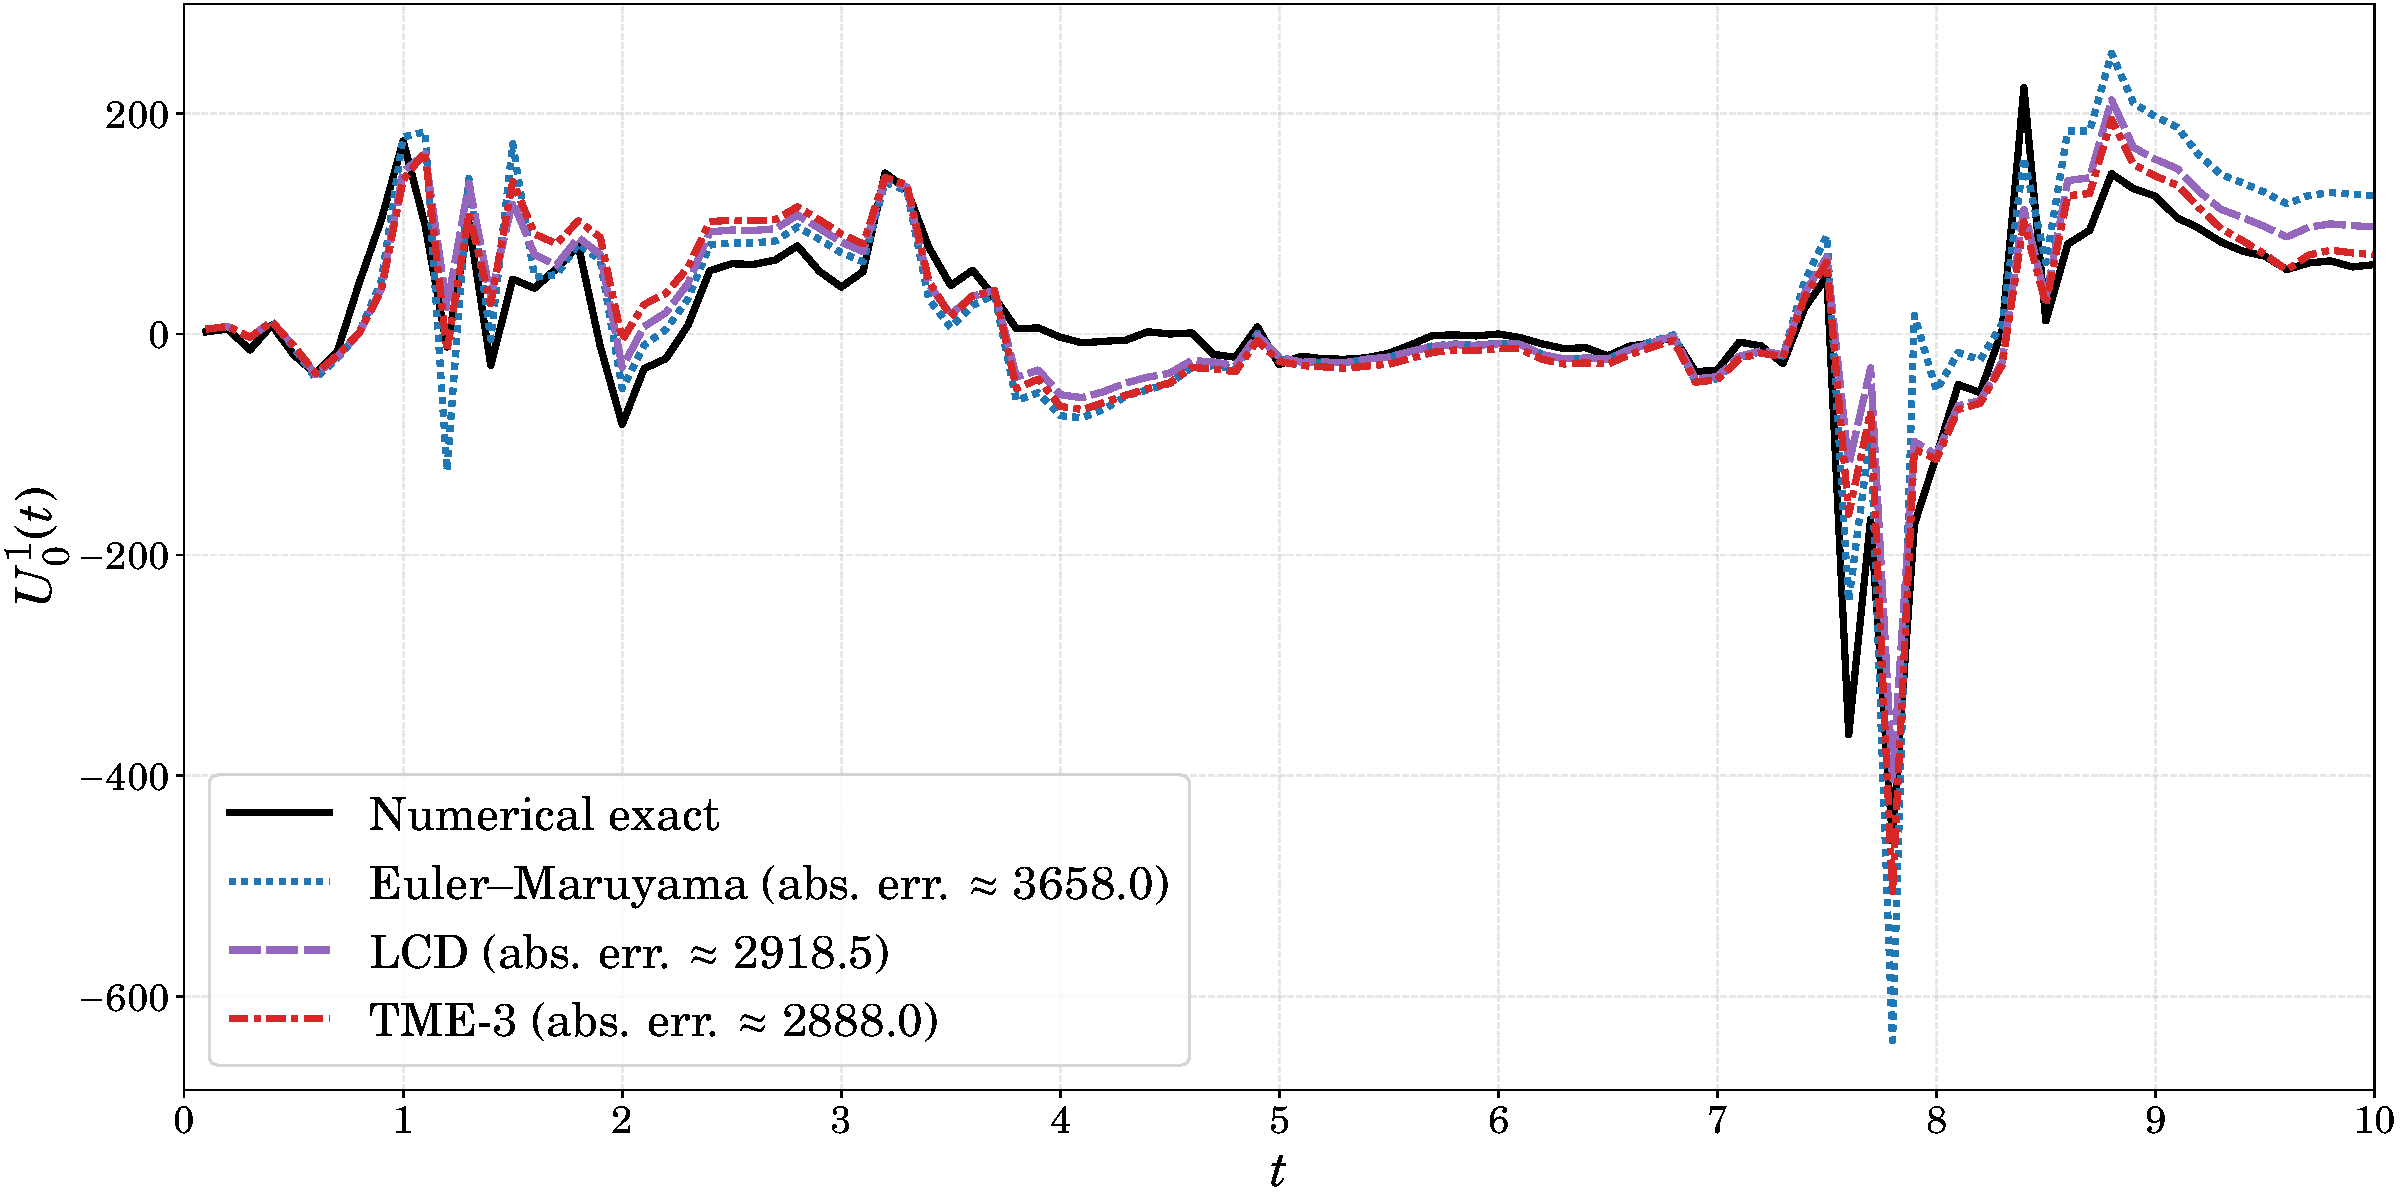
\includegraphics[width=.95\linewidth]{figs/disc-err_dgp_m12}
	\caption{Comparison of different discretisation schemes on the \matern $\nu=1\,/\,2$ SS-DGP defined in Example~\ref{example:ssdgp-m12}, where we let parameters $\ell_2=\ell_3=1$ and $\sigma_2=\sigma_3=0.1$. The numbers in the legend are the cumulative absolute errors with respect to the (numerically) exact discretisation.}
	\label{fig:disc-err-dgp-m12}
\end{figure}

Figure~\ref{fig:disc-err-dgp-m12} illustrates a comparison amongst the Euler--Maruyama, TME, and LCD methods on a \matern SS-DGP. On this example, both LCD and TME methods outperform Euler--Maruyama substantially, especially in the ``high-frequency'' portions of this SDE trajectory.

\subsection*{Exact simulation methods}

Apart from discretisation-based simulations, there also exist exact simulation methods~\citep{Beskos2005, Kessler2012, Blanchet2020}. Although these methods can avoid the discretisation errors, they are usually limited to specific types of SDEs, which may not apply to all SS-DGPs. As an example, the method introduced by~\citet{Beskos2005} requires that the dispersion coefficient be constant, which is usually not the case in SS-DGPs.

Finally, it is worth noting that each sub-SDE in Equation~\eqref{equ:ss-dgps-sde} is a linear SDE conditionally on its parent GPs. Hence, we could borrow the idea of Gibbs sampling~\citep{Robert2004} in order to sample from $U^i_{j_i}$ for $i=L,L-1,\ldots, 1$. While this method was not implemented in the context of this thesis, it is likely to improve on the LCD method and will therefore be a subject of future work.

\section{Deep \matern processes}
\label{sec:deep-matern}
In this section, we present SS-DGPs that are constructed in the Mat\'{e}rn sense. Specifically, we choose the SDE coefficients in Equation~\eqref{equ:ss-dgps-sde-split} in such a way that each GP element is a \matern GP when conditioned on its parent GPs. 

Let us start by considering linear SDEs of the form
%
\begin{equation}\label{equ:matern-linear-sde}
	\diff U(t) = A \, U(t) \diff t+ B \diff W(t),
\end{equation}
%
where the initial condition $U(t_0) \sim \mathrm{N}(0, P_0)$ is a Gaussian random variable, and the Wiener process $W\colon \T\to\R$ takes value in $\R$. Let $\nu \in \big\lbrace \frac{1}{2}, \frac{3}{2}, \ldots \big\rbrace$ and $\gamma = \nu + \frac{1}{2}$. Suppose that the state $U\colon \T \to \R^\gamma$ verifies 
\begin{equation}
	U(t) = 
	\begin{bmatrix}
	\overline{U}(t) & \frac{\diff\overline{U}}{\diff t}(t) & \cdots & \frac{\diff^{\gamma-1}\overline{U}}{\diff t^{\gamma-1}}(t) 
	\end{bmatrix}^\trans,
	\label{equ:gp-matern-state}
\end{equation}
and that the coefficients in Equation~\eqref{equ:matern-linear-sde} are given by
%
\begin{equation}
	A = 
	\begin{bmatrix}
		0 & 1 &   &\\
		  & 0 & 1 &\\
		\vdots & & \ddots &\\
		-\binom{\gamma}{0} \kappa^\gamma & -\binom{\gamma}{1} \kappa^{\gamma-1} & \cdots & -\binom{\gamma}{\gamma-1} \kappa
	\end{bmatrix}, \quad 
	B = 
	\begin{bmatrix}
		0 \\
		0\\
		\vdots\\
		\frac{\sigma \varGamma(\gamma) \, (2\,\kappa)^{\gamma - \frac{1}{2}}}{\sqrt{\varGamma(2\,\gamma-1)}}
	\end{bmatrix},
	\label{equ:matern-sde-coeffs}
\end{equation}
%
where $\kappa = \sqrt{2 \, \nu} \, / \, \ell$. Furthermore, suppose that the initial covariance $P_0$ solves the corresponding Lyapunov equation (see, Equation~\eqref{equ:lyapunuv}) of the SDE. Then the process $\overline{U} \colon \T \to \R$ in Equation~\eqref{equ:gp-matern-state} is a zero-mean Mat\'{e}rn GP with the covariance function $C_{\mathrm{Mat.}}$ defined in Equation~\eqref{equ:cov-matern}~\citep{Simo2013SSGP, Solin2016}.

\begin{remark}
	The matrix $A$ in Equation~\eqref{equ:matern-sde-coeffs} is Hurwitz~\citep{Khalil2002} as all its eigenvalues have strictly negative real part. However, $A$ is prone to be ill-conditioned if $\nu$ is large, resulting in numerically unstable SDEs. This can be addressed by using balancing algorithms~\citep{Osborne1960, Parlett1971}. 
\end{remark}

Based on the aforementioned \matern SDE representation, we can now construct \matern SS-DGPs by choosing their coefficients $A^i$ and $B^i$ for $i=1,\ldots,L$, as per Equation~\eqref{equ:matern-sde-coeffs}. As an example, suppose that the $i$-th GP element $U^i_{j_i}\in\R^{\gamma}$ in Equation~\eqref{equ:ss-dgps-sde-split} has two parents $U^m_{i}\colon \T\to\R^{d_m}$ and $U^n_{i}\colon \T\to\R^{d_n}$, that encode the length scale and the magnitude parameters, respectively. Then, we can select two suitable transformation functions $g_m \colon \R^{d_m} \to \R_{>0}$ and $g_n \colon \R^{d_n} \to \R_{>0}$, and let 
%
\begin{equation}
	\ell_i(t) = g_m\bigl( U^m_{i}(t) \bigr)
	\label{equ:ss-dgp-ell}
\end{equation}
%
and
%
\begin{equation}
	\sigma_i(t) = g_n\big(U^n_{i}(t)\big).
	\label{equ:ss-dgp-sig}
\end{equation} 
%
Under these notations, the coefficient $A^i$ of $U^i_{j_i}$ reads
%
\begin{equation}
		A^i(t; \mathcal{U}^i) = A^i\big( U^m_{i}(t)\big) = \begin{bmatrix}
		0 & 1 &   &\\
		& 0 & 1 &\\
		\vdots & & \ddots &\\
		-\binom{\gamma}{0} \kappa^\gamma_i(t) & -\binom{\gamma}{1} \kappa^{\gamma-1}_i(t) & \cdots & -\binom{\gamma}{\gamma-1} \kappa_i(t)
		\end{bmatrix},
\end{equation}
%
where $\kappa_i(t) = \sqrt{2 \, \nu} \, / \, \ell_i(t)$. Likewise, one can derive the coefficient $B^i(t; \mathcal{U}^i) = B^i\big( U^m_{i}(t), U^n_{i}(t) \big) = \begin{bmatrix}
	0 & 0 & \cdots & \sigma_i(t) \, \varGamma(\gamma) \, (2\,\kappa_i(t))^{\gamma - \frac{1}{2}}\, (\varGamma(2\,\gamma-1))^{\frac{1}{2}}
\end{bmatrix}^\trans \in \R^{\gamma}$.

Transformation functions should also be chosen regular enough so that the solution of the related SDE is well-defined (see, Section~\ref{sec:ssdgps-solution}). For example, in~\citet{Zhao2020SSDGP, Zhao2021RSSGP}, we use $g(u) = \exp(u)$, $g(u) = \arctan(u) + \pi \, / \, 2$, or $g(u) = \log(1 + \exp(u))$.

SDEs of Mat\'{e}rn SS-DGPs are time-homogeneous by construction (i.e., the coefficients $A^i$ and $B^i$ for $i=1,2,\ldots,L$ do not explicitly depend on time). Provided that the transformation functions are chosen suitably as per~\citet[][Definition~7.1.1]{Oksendal2003}, the \matern SS-DGPs are then It\^{o} diffusions. This can bring many useful features, such as the strong Markov property~\citep{Ikeda1992}. 

In the following, we give some concrete examples of Mat\'{e}rn SS-DGPs and plot a few of their simulations. 

\begin{example}[Mat\'{e}rn $\nu=1\,/\,2$ SS-DGP with three GP elements]
	\label{example:ssdgp-m12}
	Let $\nu=1\, / \, 2$. Consider the following SDEs
	\begin{equation}
		\begin{split}
			\diff U^1_0(t) &= -\frac{1}{\ell_1(t)}\,U^1_0(t) \diff t + \frac{\sqrt{2} \, \sigma_1(t)}{\sqrt{\ell_1(t)}} \diff W^1(t),\\
			\diff U^2_1(t) &= -\frac{1}{\ell_2}\,U^2_1(t) \diff t + \frac{\sqrt{2} \, \sigma_2}{\sqrt{\ell_2}} \diff W^2(t),\\
			\diff U^3_1(t) &= -\frac{1}{\ell_3}\,U^3_1(t) \diff t + \frac{\sqrt{2} \, \sigma_3}{\sqrt{\ell_3}} \diff W^3(t),
		\end{split}
		\label{equ:ss-dgp-m12}
	\end{equation}
	where $\ell_1(t) = g\big( U^2_1(t) \big)$ and $\sigma_1 = g\big( U^3_1(t) \big)$ are the length scale and magnitude of $U^1_0(t)$, respectively. The solution $V(t) = \begin{bmatrix}
		U^1_0(t) & U^2_1(t) & U^3_1(t)
	\end{bmatrix}^\trans$ is said to be a Mat\'{e}rn $\nu=1\,/\,2$ SS-DGP. 
\end{example}

\begin{example}[Mat\'{e}rn $\nu=3\,/\,2$ SS-DGP with three GP elements]
	\label{example:ssdgp-m32}
	Let $\nu= 3 \, / \, 2$. Consider the following SDEs
	\begin{equation}
		\begin{split}
			\diff U^1_0(t) &= 
			\begin{bmatrix}
				0 & 1\\
				-\big(\frac{\sqrt{3}}{\ell_1(t)}\big)^2 & \frac{-2 \,\sqrt{3}}{\ell_1(t)}
			\end{bmatrix} \, U^1_0(t) \diff t + 
			\begin{bmatrix}
				0 \\
				2\,\sigma_1(t) \, \big(\frac{\sqrt{3}}{\ell_1(t)}\big)^{\frac{3}{2}}
			\end{bmatrix} \diff W^1(t), \\
			\diff U^2_1(t) &= 
			\begin{bmatrix}
				0 & 1\\
				-\big(\frac{\sqrt{3}}{\ell_2}\big)^2 & \frac{-2 \,\sqrt{3}}{\ell_2}
			\end{bmatrix} \, U^2_1(t) \diff t + 
			\begin{bmatrix}
				0 \\
				2\,\sigma_2 \, \big(\frac{\sqrt{3}}{\ell_2}\big)^{\frac{3}{2}}
			\end{bmatrix} \diff W^2(t), \\
			\diff U^3_1(t) &= 
			\begin{bmatrix}
				0 & 1\\
				-\big(\frac{\sqrt{3}}{\ell_3}\big)^2 & \frac{-2 \,\sqrt{3}}{\ell_3}
			\end{bmatrix} \, U^3_1(t) \diff t + 
			\begin{bmatrix}
				0 \\
				2\,\sigma_3 \, \big(\frac{\sqrt{3}}{\ell_3}\big)^{\frac{3}{2}}
			\end{bmatrix} \diff W^3(t), 
		\end{split}
	\end{equation}
	where $U^1_0(t) = \begin{bmatrix}
		\overline{U}^1_0(t) & \frac{\diff\overline{U}^1_0}{\diff t}(t)
	\end{bmatrix}^\trans$, and similarly for $U^2_1(t)$ and $U^3_1(t)$. The length scale and magnitude of $U^1_0(t)$ are given by $\ell_1(t) = g\big( U^2_1(t) \big)$ and $\sigma_1 = g\big( U^3_1(t) \big)$, respectively, for $g\colon \R^2 \to \R_{>0}$. The solution $V(t) = \begin{bmatrix}
	U^1_0(t) & U^2_1(t) & U^3_1(t)
	\end{bmatrix}^\trans$ is said to be a Mat\'{e}rn $\nu=3\,/\,2$ SS-DGP. 
	
	It is worth noting that for this model the Euler--Maruyama scheme gives a singular discretisation covariance.
\end{example}

\begin{figure}[t!]
	\centering
	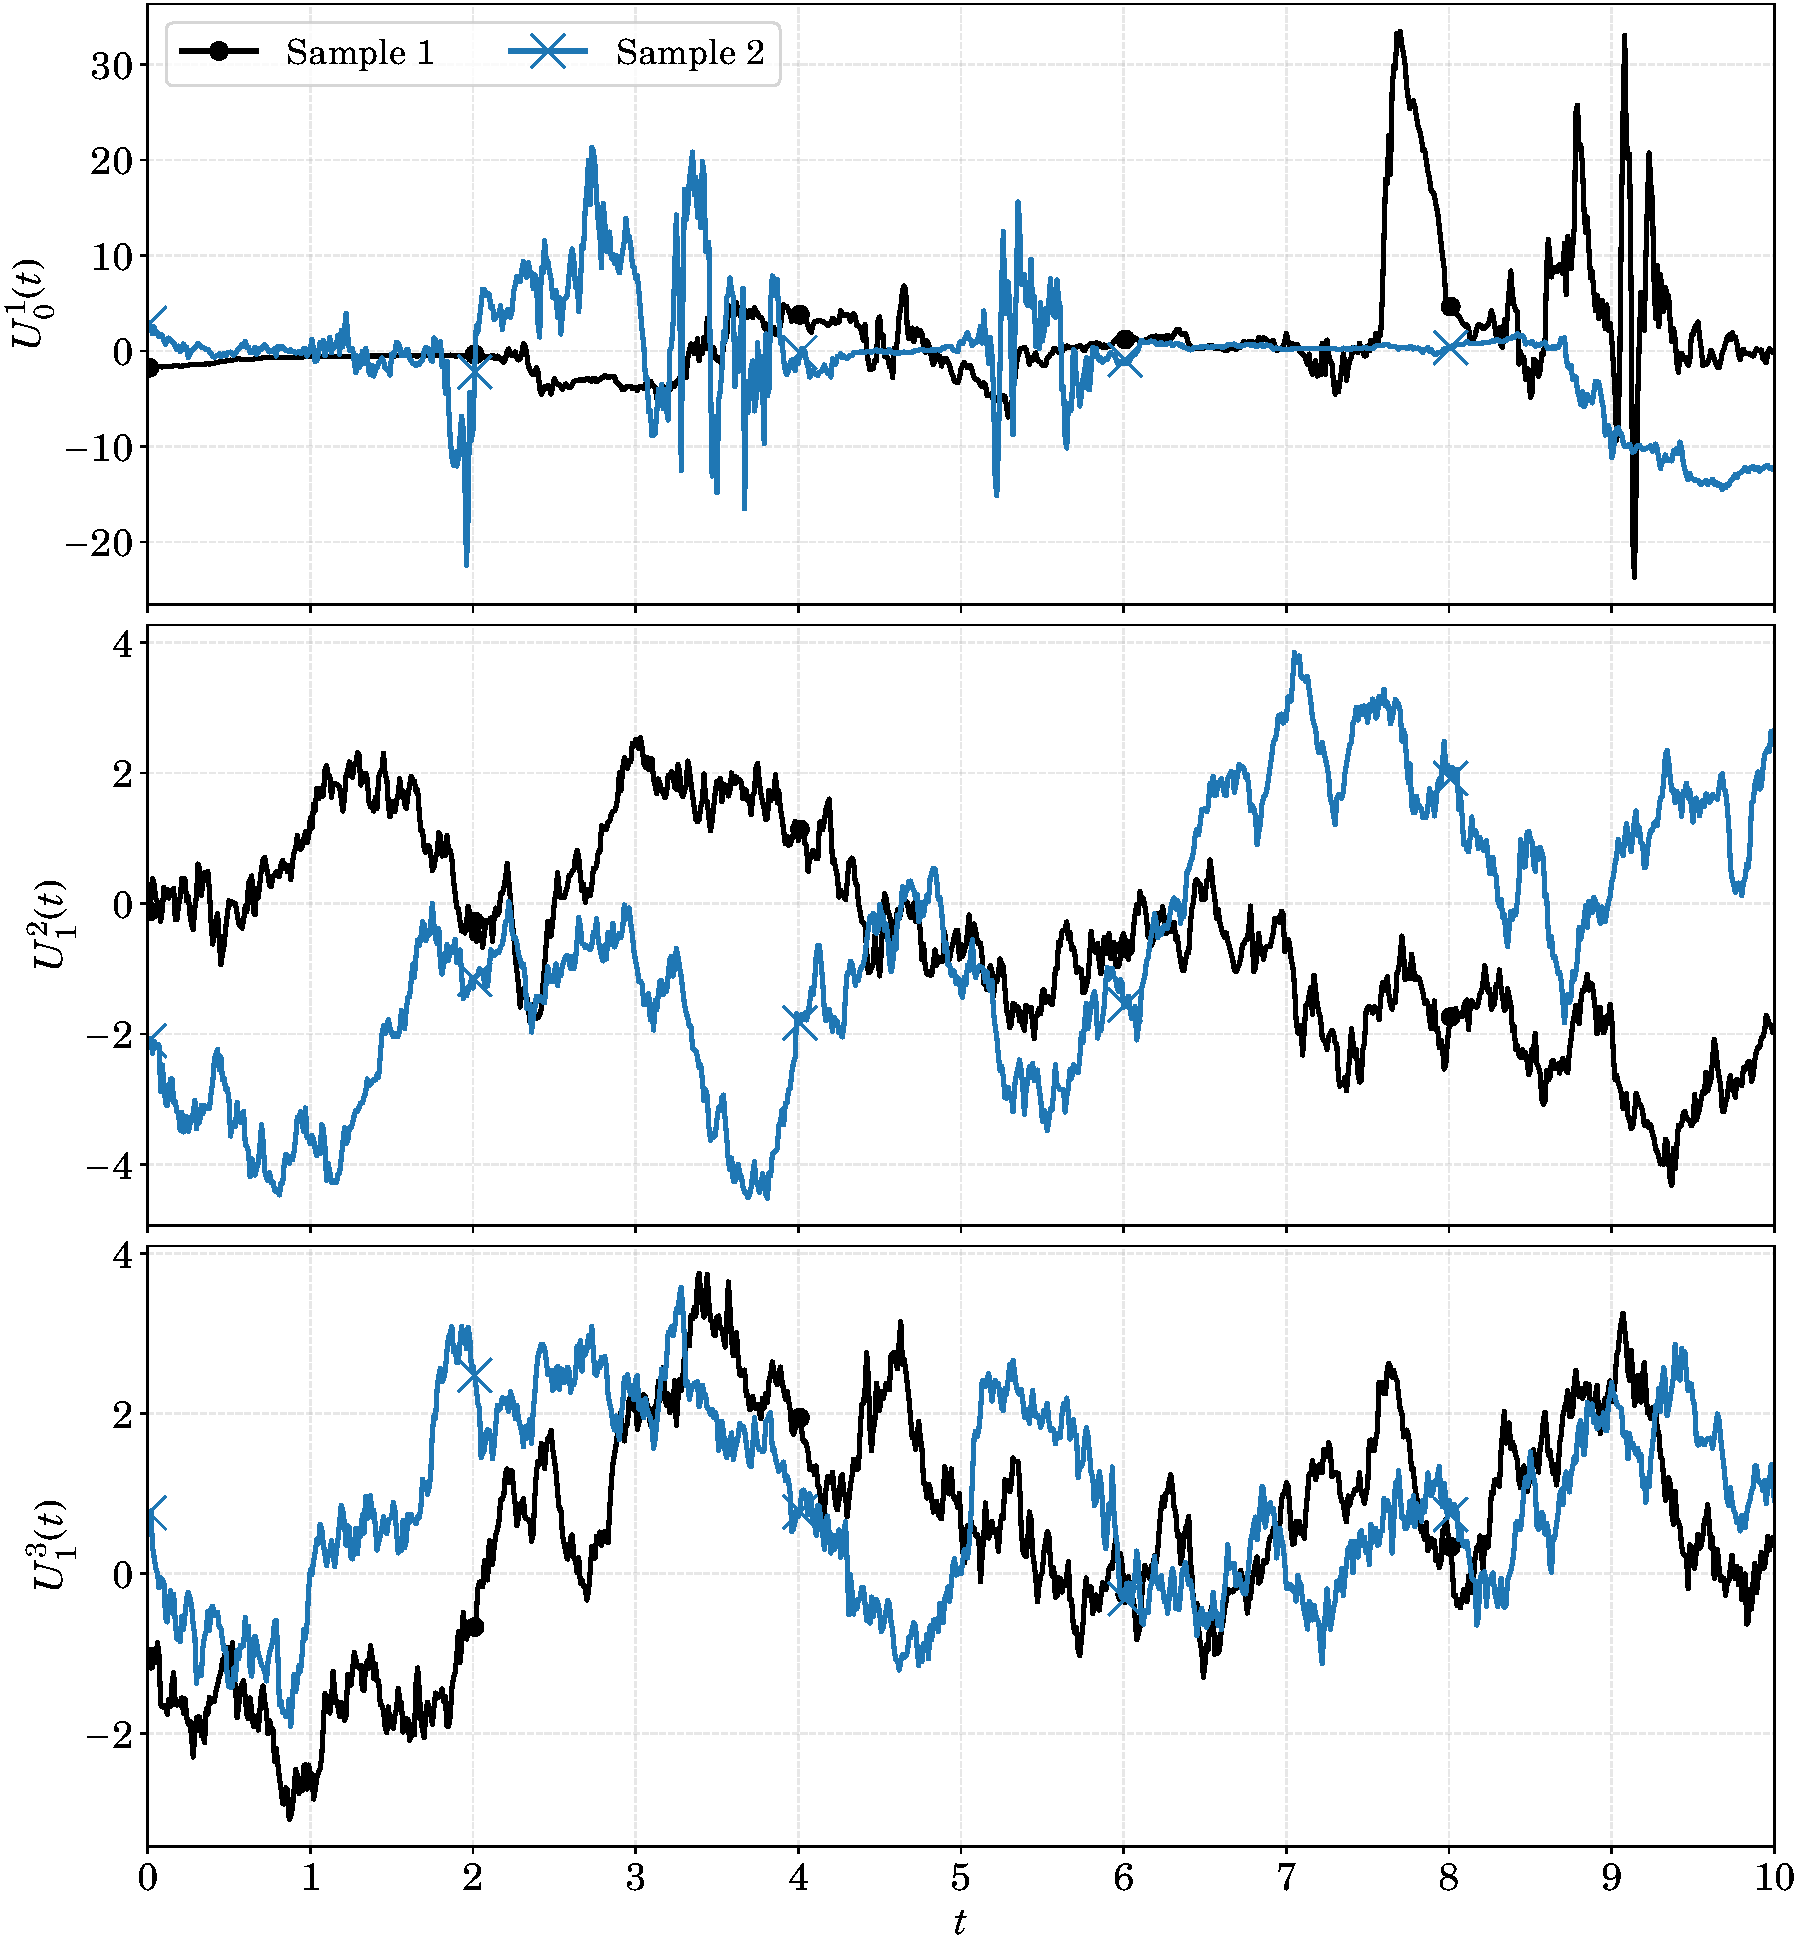
\includegraphics[width=.95\linewidth]{figs/samples_ssdgp_m12}
	\caption{This figure shows two samples (plotted in different colours and markers) drawn from the Mat\'{e}rn $\nu=1\,/\,2$ SS-DGP defined in Example~\ref{example:ssdgp-m12}.}
	\label{fig:ssdgp-m12-samples}
\end{figure}
%
\begin{figure}[t!]
	\centering
	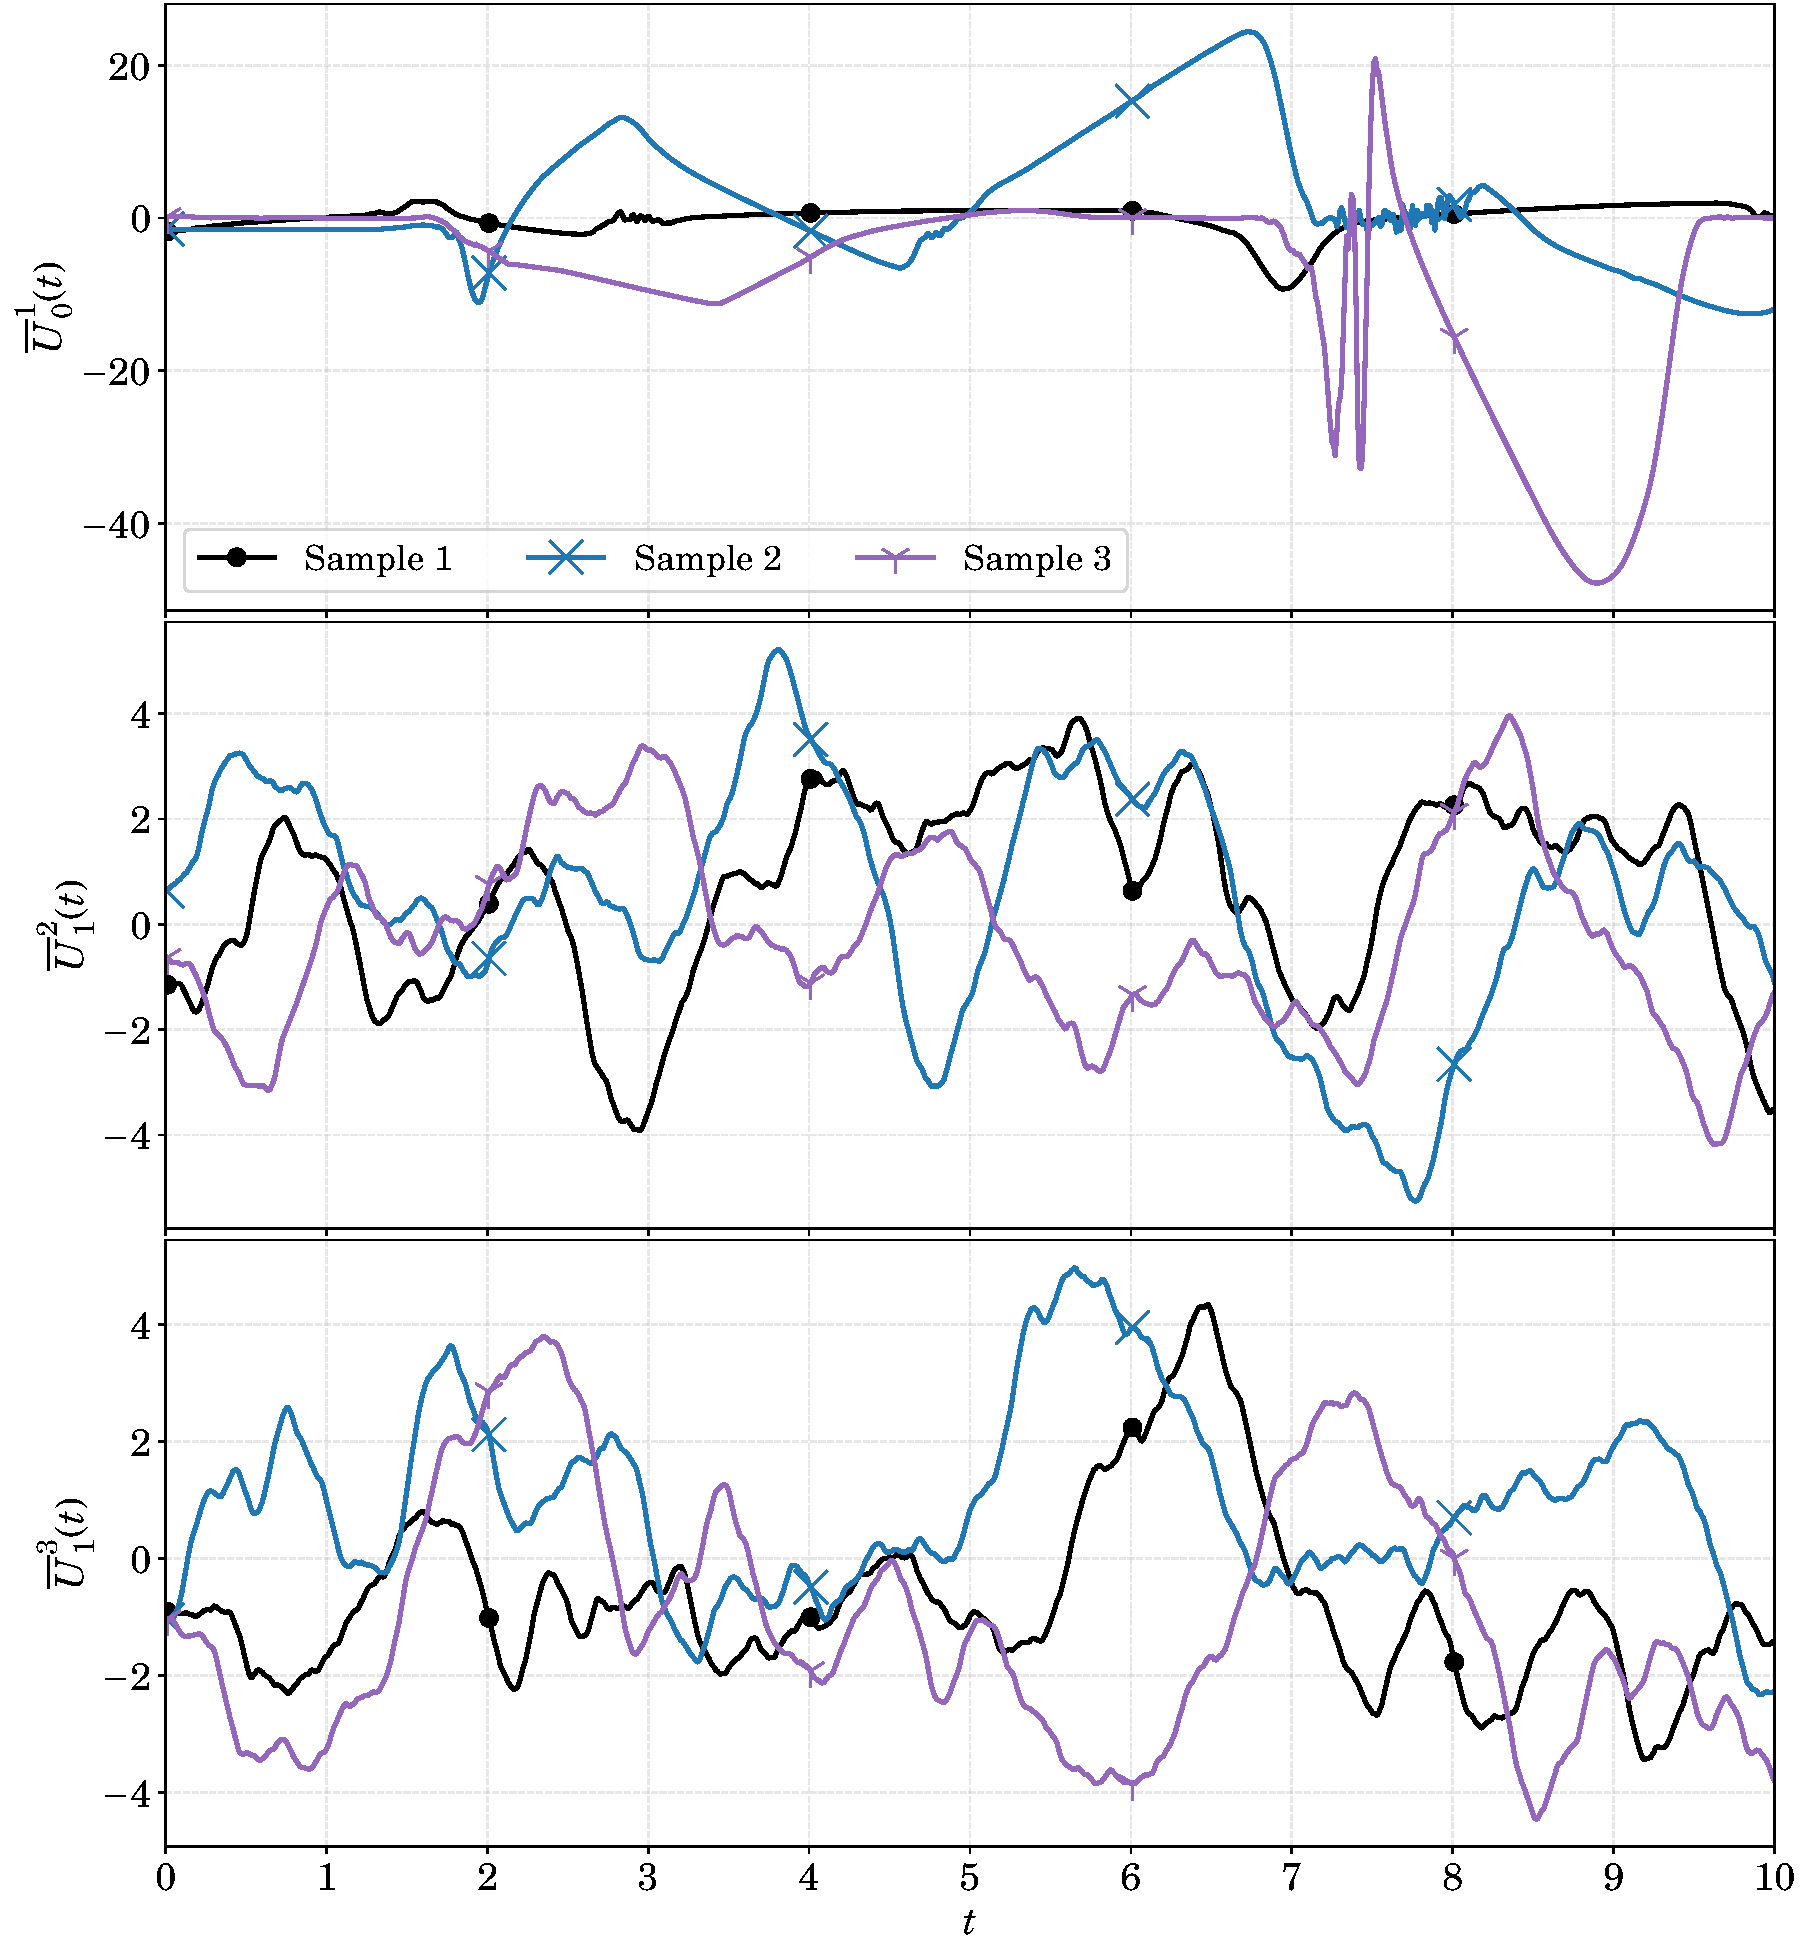
\includegraphics[width=.95\linewidth]{figs/samples_ssdgp_m32}
	\caption{This figure shows three samples (plotted in different colours and markers) drawn from the Mat\'{e}rn $\nu=3\,/\,2$ SS-DGP defined in Example~\ref{example:ssdgp-m32}.}
	\label{fig:ssdgp-m32-samples}
\end{figure}

The Examples~\ref{example:ssdgp-m12} and~\ref{example:ssdgp-m32} feature Mat\'{e}rn SS-DGPs with only three GP elements. This hierarchy/depth can be continued further to represent higher degrees of non-stationarity. 

Figures~\ref{fig:ssdgp-m12-samples} and~\ref{fig:ssdgp-m32-samples} illustrate a few samples drawn from the Mat\'{e}rn SS-DGPs defined in Examples~\ref{example:ssdgp-m12} and~\ref{example:ssdgp-m32}, respectively. More specifically, for the Mat\'{e}rn $\nu=1\,/\,2$ SS-DGP in Example~\ref{example:ssdgp-m12} we use $\ell_2=\ell_3=\sigma_2=\sigma_3=2$ and $g(u) = \exp(u)$, while for the Mat\'{e}rn $\nu=3\,/\,2$ SS-DGP in Example~\ref{example:ssdgp-m32} we use $\ell_2=\ell_3=0.5$, $\sigma_2=\sigma_3=2$ and $g(u) = \exp\big( \big[ 1 \,\,0 \big] \, u \big)$. The initial states are standard Gaussian random vectors with unit covariances in both cases.

From Figures~\ref{fig:ssdgp-m12-samples} and~\ref{fig:ssdgp-m32-samples}, we can observe non-stationary in the behaviour of $U^1_0$. This results from its length scale and magnitude being driven by its parent GPs $U^2_1$ and $U^3_1$. As an example, Sample~2 (blue line) of $\overline{U}^1_0$ in Figure~\ref{fig:ssdgp-m32-samples} exhibits low-magnitude high-frequency jittering around $t\in[7, 8]$ because the length scale $g\big(\overline{U}^2_1\big)$ and magnitude $g\big(\overline{U}^3_1\big)$ are relatively small on $t\in[7, 8]$. On the other hand Sample~3 (magenta line) of $\overline{U}^1_0$ in Figure~\ref{fig:ssdgp-m32-samples} exhibits high-magnitude medium-frequency jittering around $t\in[7, 8]$ because the length scale $g\big(\overline{U}^2_1\big)$ and magnitude $g\big(\overline{U}^3_1\big)$ are relatively average and high, respectively, on $t\in[7, 8]$.

The main usefulness of this Mat\'{e}rn construction is that the resulting Mat\'{e}rn SS-DGPs can provide generic priors for modelling a wide class of continuous functions (with smoothness parameter $\gamma - 1$). These priors are flexible in the sense that they have non-stationary characteristics which can be learnt from data. In Chapter~\ref{chap:apps}, we will show some real applications of Mat\'{e}rn SS-DGPs. 

Apart from the Mat\'{e}rn construction, it is also possible to build SS-DGPs by formulating SDE coefficients in some other meaningful ways. For example, \citet{Solin2014} construct SDEs that represent quasi-periodic oscillators, and~\citet{Syama2018} parametrise SDEs with neural networks for time series forecasting.

\begin{figure}[t!]
	\centering
	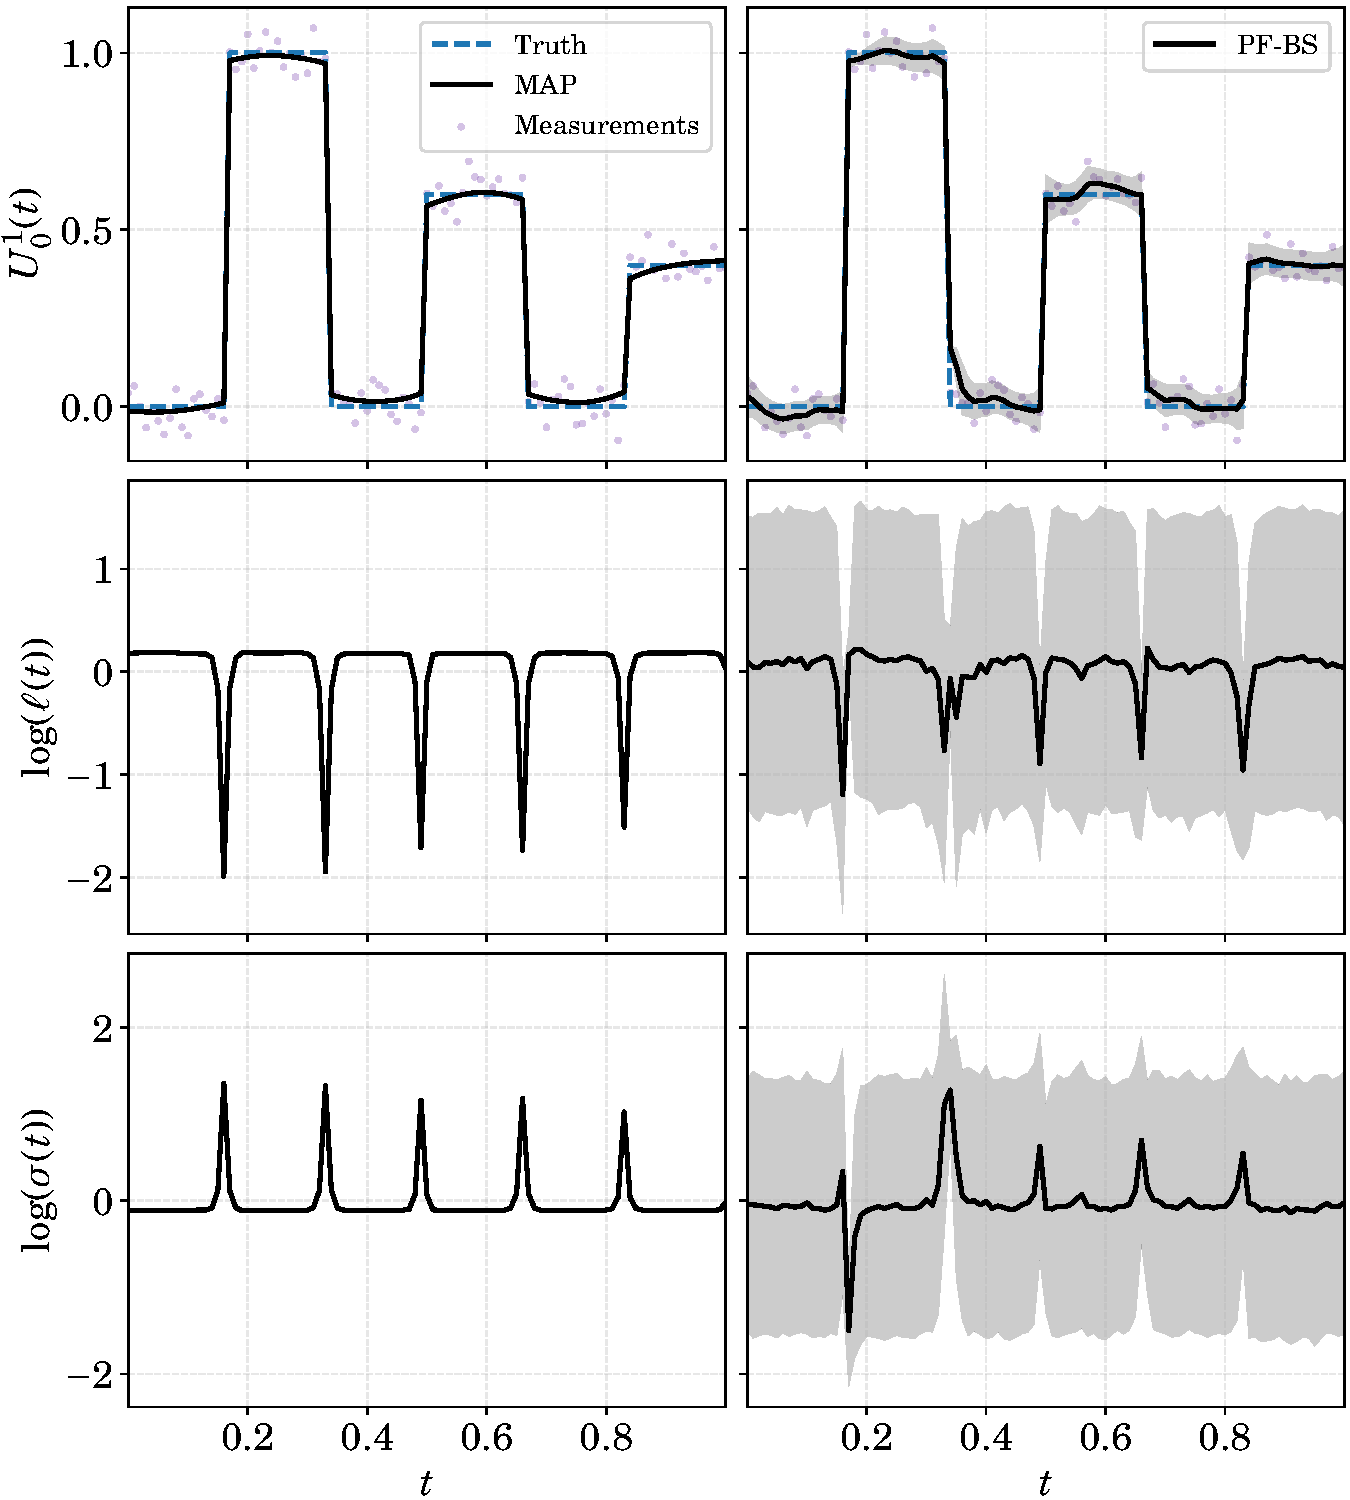
\includegraphics[width=.9\linewidth]{figs/ssdgp-reg-rect}
	\caption{Mat\'{e}rn SS-DGP regression on a rectangular signal. The first column corresponds to the MAP estimate of the SDE state, while the second column corresponds to a full posterior estimate using PF-BS (particle filter and backward simulation smoother). }
	\label{fig:ssdgp-reg-rect}
\end{figure}
%
\begin{figure}[t!]
	\centering
	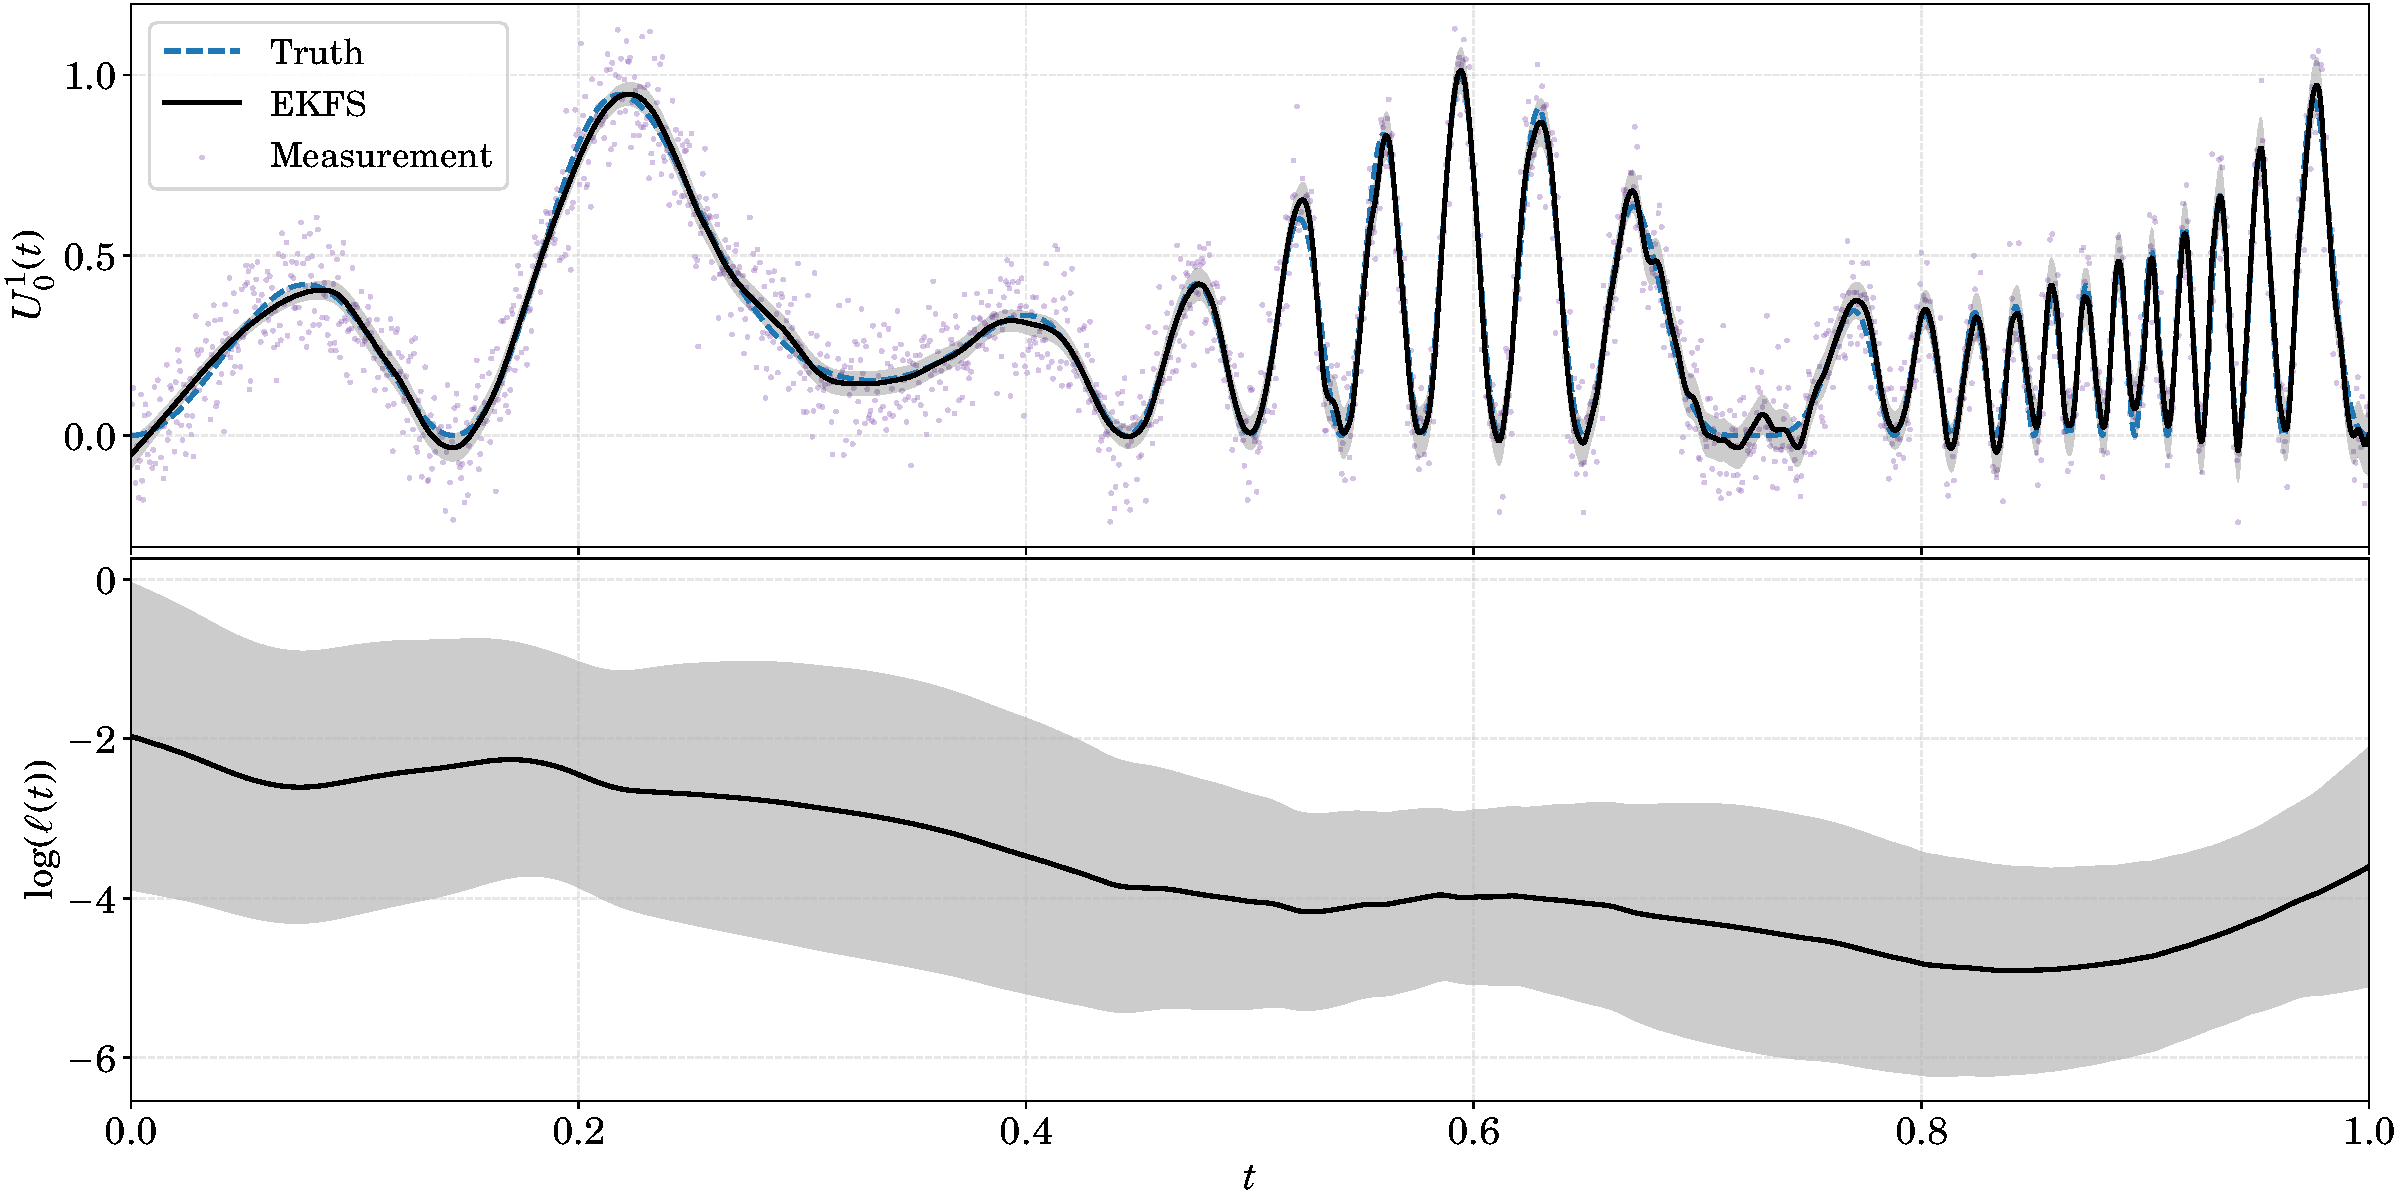
\includegraphics[width=.99\linewidth]{figs/ssdgp-reg-sine}
	\caption{Mat\'{e}rn SS-DGP regression on a composite sinusoidal signal by using EKFS (extended Kalman filter and smoother). }
	\label{fig:ssdgp-reg-sine}
\end{figure}

\section{SS-DGP Regression}
\label{sec:ssdgp-reg}
In this section, we show how to solve SS-DGP regression problems for discrete measurement data. Since SS-DGPs are characterised by SDEs, we view these problems as continuous-discrete Bayesian smoothing problems (see, Section~\ref{sec:cd-smoothing}).

Let $V \colon \T \to \R^{\sum^L_{i=1} d_i}$ be an SS-DGP defined as per Equation~\eqref{equ:ss-dgps-sde}. Suppose that we measure $V$ at $t_1, t_2,\ldots, t_T \in \T$, by a (non-linear) function $h\colon \R^{\sum^L_{i=1} d_i} \to \R^{d_y}$ and additive Gaussian noises $\xi_k\sim\mathrm{N}(0, \Xi_k)$ for $k=1,2,\ldots, T$. We consider the SS-DGP regression problem in its continuous-discrete state-space form
%
\begin{equation}
	\begin{split}
		\diff V(t) &= a(V(t)) \diff t + b(V(t)) \diff W(t), \quad V(t_0) = V_0,\\
		Y_k &= h(V_k) + \xi_k,
		\label{equ:ssdgp-regression}
	\end{split}
\end{equation}
%
where we abbreviate $V_k \coloneqq V(t_k)$. Suppose we have a set of measurements $y_{1:T} = \lbrace y_1, y_2, \ldots, y_T\rbrace $, we want to learn the (smoothing) posterior density $p_{V_k \cond Y_{1:T}}(v_k \cond y_{1:T})$ for $k=1,2,\ldots, T$, or more generally $p_{V(t) \cond Y_{1:T}}(v,t \cond y_{1:T})$, for any $t\in\T$. We can then use the methods presented in Section~\ref{sec:cd-smoothing} to solve the regression/continuous-discrete smoothing problem above. 

Thanks to the Markov property of the SS-DGP prior, we can solve this regression problem in linear computational time with respect to $T$ by leveraging Bayesian filtering and smoothing methods. This is in contrast with batch DGPs, where one often needs to solve matrix inversions of dimension $T\times T$.

In Figures~\ref{fig:ssdgp-reg-rect} and~\ref{fig:ssdgp-reg-sine}, we plot some SS-DGP regression examples taken from~\citet{Zhao2020SSDGP}. Compared to the GP regression shown in Figure~\ref{fig:gp-fail}, we can see the advantages of SS-DGPs for fitting irregular data. Also, the estimated length scale and magnitude parameters can explain well the changes of regime in the data generating process. 

It would be also possible to extend SS-DGP regression to classification by modifying the measurement model in Equation~\eqref{equ:ssdgp-regression} accordingly~\citep{Neal1998, Carl2006GPML, Garcia2019}. For example, we can assume that the measurement follows a categorical distribution, with parameters determined by the SS-DGP states~\citep{Carl2006GPML}.

\section{Identifiability analysis of Gaussian approximated SS-DGP regression}
\label{sec:identi-problem}
Gaussian filters and smoothers (GFSs, see, Section~\ref{sec:gaussian-filter-smoother}) are widely used classes of Bayesian filters and smoothers. Moreover, \citet{Zhao2020SSDGP} show that GFSs are particularly efficient for solving SS-DGP regression problems. However, for a certain class of SS-DGPs, GFSs cannot identify (i.e., estimate the posterior density of) their state components as $t\to\infty$. More specifically, in this section, we show how -- under some weak assumptions on the SS-DGP regression model coefficients -- the posterior (cross-)covariance estimates of the regression problem solutions at the measurements times $t_k$ collapse to $0$ as $k\to\infty$.

\begin{figure}[t!]
	\centering
	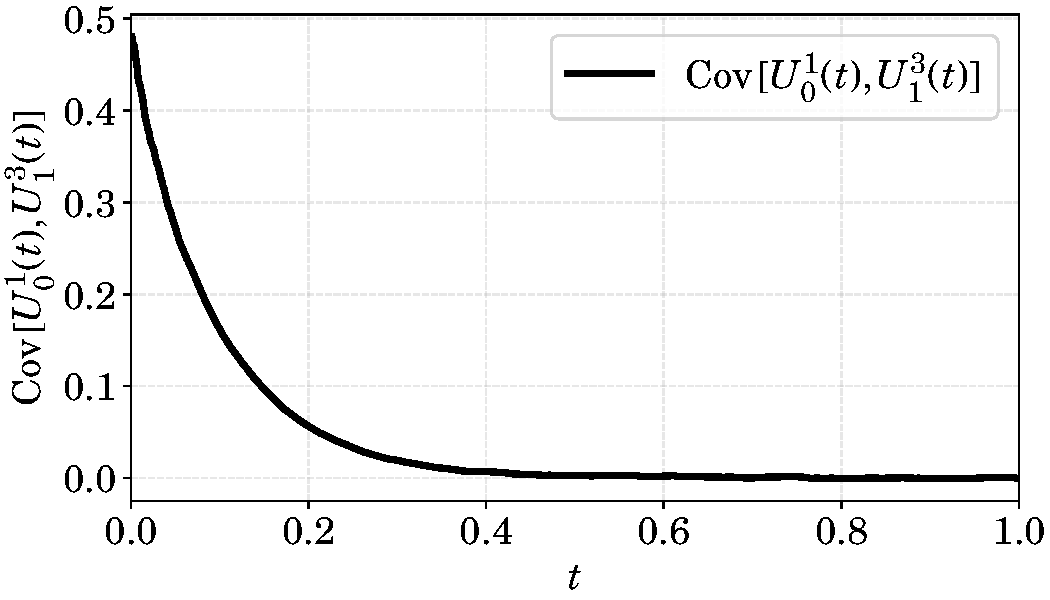
\includegraphics[width=.7\linewidth]{figs/vanishing-cov}
	\caption{Evolution of $\covbig{U^1_0(t), U^3_1(t)}$ in Example~\ref{example:ssdgp-m12}, estimated by 20,000 independent Monte Carlo runs. Parameters are $\ell_2=\ell_3=\sigma_2=\sigma_3=0.1$, and the initial $\covbig{U^1_0(0), U^3_1(0)}=0.5$. We observe that the covariance (numerically) converges to zero monotonically as $t$ grows.}
	\label{fig:ssdgp-vanishing-cov}
\end{figure}

To explain the problem in short, let us suppose that we have an SS-DGP regression model with the SDE given by Example~\ref{example:ssdgp-m12}, and that we measure the first GP element $U^1_0$ with additive Gaussian noises. Further suppose that we apply GFSs (see, Algorithm~\ref{alg:gfs}) to solve the regression problem. It turns out that this SDE has a vanishing $\covbig{U^1_0(t), U^3_1(t)} \to 0$ as $t\to\infty$ (see, Figure~\ref{fig:ssdgp-vanishing-cov} for a numerical illustration), and that the GFS estimated posterior $\covbig{U^1_0(t_k), U^3_1(t_k) \cond y_{1:k}}$ vanishes to zero as $k\to \infty$ too. Consequently, the Kalman gain for the component $U^3_1$ converges to zero as $k\to\infty$. This means that the posterior distribution of $U^3_1$ estimated by GFSs will use no information from measurements as $k\to\infty$.

In order to formulate the problem, we limit ourselves to a class of SS-DGP regression models for which the dispersion term of the observed GP element is parametrised by another GP element. Formally, we consider $U^1_0\colon \T \to \R$ and $U^2_1 \colon \T \to \R$ that are the solutions of the pair of SDEs
%
\begin{equation}
	\begin{split}
		\diff U^1_0(t) &= A^1( \psi(t) ) \, U^1_0(t) \diff t + B^1\big(\psi(t), U^2_1(t)\big) \diff W^1(t),\\
		\diff U^2_1(t) &= A^2(\varphi(t)) \, U^2_1(t) \diff t + B^2(\varphi(t)) \diff W^2(t),
		\label{equ:ident-sde}
	\end{split}
\end{equation}
%
on a filtered probability space $(\Omega, \FF, \FF_t, \PP )$, where the initial conditions, the processes $\psi \colon \T \to \R$ and $\varphi \colon \T \to \R$, and the Wiener processes $W^1 \colon \T \to \R$ and $W^2 \colon \T \to \R$ are mutually independent.
\begin{remark}
	Note that the index $2$ on $U^2_1$ is arbitrary as the definition of a DGP is invariant of reindexing of its components (see, Definition~\ref{def:dgp}).
\end{remark}

\begin{remark}
	The SDEs given by Equation~\eqref{equ:ident-sde} represent a class of SS-DGPs for which an inner GP element $U^2_1$ parametrises the dispersion term of the measured GP element $U^1_0$. Since the parents of $U^1_0$ and $U^2_1$ are not necessarily Gaussian (but are instead conditional Gaussian), we generically name their parents $\psi$ and $\varphi$ which can be any well-defined processes. As an example, in the left figure of Figure~\ref{fig:dgp-examples-graph}, one can imagine $\psi$ as the representation of $U^3_1$, $U^6_3$, and $U^7_3$, while $\varphi$ as the representation of $U^4_2$ and $U^5_2$.
\end{remark}

Let the random variables
%
\begin{equation}
	Y_k = U^1_0(t_k) + \xi_k, \quad \xi_k \sim \mathrm{N}(0, \Xi_k),
	\label{equ:ident-y}
\end{equation}
%
for $k=1,2,\ldots$ stand for the measurements at time $t_1, t_2, \ldots$, and assume that $\inf_k \lbrace t_k - t_{k-1} \colon k=1,2,\ldots\rbrace > 0$.

We use the following assumptions. 

\begin{assumption}
	\label{assump:ssdgp-ident-solution}
	The coefficients $A^1 \colon \R \to \R_{<0}$, $B^1 \colon \R \times \R \to \R$, $A^2 \colon \R \to \R_{<0}$, $B^2\colon \R \to \R$, and the initial conditions are chosen regular enough so that the weak uniqueness (see, Definition~\ref{def:weakly-unique}) holds for the SDE in Equation~\eqref{equ:ident-sde} .
\end{assumption}

\begin{assumption}
	\label{assump:ssdgp-ident-init}
	The components $U^1_0$ and $U^2_1$ at the initial time $t_0$ satisfy
	$\expecbig{\absbig{U^1_0(t_0)}} < \infty$, $\expecbig{ \absbig{U^2_1(t_0)}} < \infty$, and $\expecbig{ \absbig{U^1_0(t_0) \, U^i_1(t_0)}} < \infty$.
\end{assumption}

\begin{assumption}
	\label{assump:ssdgp-ident-neg}
	There exists constants $c_{A^1}<0$ and $c_{A^2}<0$ such that $\PP$-almost surely the processes $(A^1 \circ \psi)(t) \leq c_{A^1}$ and $(A^2 \circ \varphi)(t) \leq c_{A^2}$ for all $t\in\T$. 
\end{assumption}

\begin{assumption}
	\label{assump:ssdgp-ident-bound-A-B}
	There exist constants $c_A > 0$ and $c_B>0$ such that, for all $t \in \T$, $\expecbig{\big( A^1(\psi(t))\,U^1_0(t) \big)^2} \leq c_A$ and $\expecbig{\big( B^1\big(\psi(t), U^2_1(t)\big) \big)^2} \geq c_B$.
\end{assumption}

\begin{assumption}
	\label{assump:ssdgp-ident-bound-R}
	There exists $\Xi_{\mathrm{inf}} > 0$ such that for every $k=1,2,\ldots$, either $\Xi_k > \Xi_{\mathrm{inf}}$ or $\Xi_k = 0$.
\end{assumption}

Assumption~\ref{assump:ssdgp-ident-solution} ensures SDEs~\eqref{equ:ident-sde} be well-defined. Assumption~\ref{assump:ssdgp-ident-init} postulates absolute integrability of the initial conditions which is used in the proof of Lemma~\ref{lemma:vanishing-prior-cov}. Assumption~\ref{assump:ssdgp-ident-bound-A-B} aims to yield a positive lower bound for $\varrbig{U^1_0(t)}$ as used in Corollary~\ref{corollary:var-f-bound}. 

Assumption~\ref{assump:ssdgp-ident-neg} is the key assumption to have the prior covariance vanishing. This assumption is pragmatic because it ensures that the mean of $U^1_0$ and $U^2_1$ shrinks to zero over time. Also, if one considers $-1 \,/\, A^1$ and $-1 \, / \, A^2$ as length scales, then this assumption guarantees their positivity.

\begin{lemma}
	\label{lemma:vanishing-prior-cov}
	Under Assumptions~\ref{assump:ssdgp-ident-solution} to~\ref{assump:ssdgp-ident-neg}, 
	%
	\begin{equation}
		\lim_{t\to\infty} \covbig{U^1_0(t), U^2_1(t)} = 0.
		\label{equ:vanish-cov-0}
	\end{equation}
	%
\end{lemma}
\begin{proof}
	By It\^{o}'s formula and the law of total expectation, one can find that 
	%
	\begin{align}
		\covbig{U^1_0(t), U^2_1(t)} &= \expecBig{\expecbig{U^1_0(t_0) \, U^2_1(t_0) \cond \psi(t_0), \varphi(t_0)} \expp^{\int^t_{t_0} A^1( \psi(s)) + A^2( \varphi(s)) \diff s}} \nonumber\\
		&\quad-\expecBig{\expecbig{U^1_0(t_0) \cond \psi(t_0)} \expp^{\int^t_{t_0} A^1( \psi(s)) \diff s }} \label{equ:vanish-cov-eq1}\\
		&\qquad\times\expecBig{\expecbig{U^2_1(t_0) \cond \varphi(t_0)} \expp^{\int^t_{t_0} A^2( \varphi(s)) \diff s }}.\nonumber
	\end{align}
	%
	Next, knowing that $A^1 \circ \psi$ and $A^2 \circ \varphi$ are upper bounded by Assumption~\ref{assump:ssdgp-ident-neg}, we can then apply the triangle inequality and conditional Jensen's inequality~\citep[][Theorem 8.20]{AchimKlenke2014} to bound the three terms in the equation above. As an example, the first term admits
	%
	\begin{equation}
		\begin{split} &\absBig{\expecBig{\expecbig{U^1_0(t_0) \, U^2_1(t_0) \cond \psi(t_0), \varphi(t_0)} \, \expp^{\int^t_{t_0} A^1( \psi(s)) + A^2(\varphi(s)) \diff s }}}\\
		&\leq \expecBig{\absbig{\expecbig{U^1_0(t_0) \, U^2_1(t_0) \cond \psi(t_0), \varphi(t_0)}} \, \absbig{\expp^{\int^t_{t_0} A^1( \psi(s)) + A^2(\varphi(s)) \diff s }}} \\
		&\leq \expecBig{\absbig{U^1_0(t_0) \, U^2_1(t_0) }} \, \expp^{(c_{A^1} + c_{A^2}) \, (t - t_0)}.
		%&\leq \sqrt{\expecbig{\big(U^1_0(t_0) \big)^2} \, \expecbig{\big(U^2_1(t_0) \big)^2}} \, e^{(c_{A^1} + c_{A^2}) \, (t - t_0)},
		\label{equ:ssdgp-identi-lemma-cov-ineq}
		\end{split}
	\end{equation}
	%
% 	Next, by using Jensen's inequality and H\"{o}lder's inequality, we can form two-sided bounds for the three expectations terms in Equation~\eqref{equ:vanish-cov-eq1}. For instance, 
% 	%
% 	\begin{equation}
% 		\begin{split}
% 			&\absBig{\expecBig{\expecbig{U^1_0(t_0) \cond \psi(t_0)} e^{\int^t_{t_0} A^1( \psi(s)) \diff s }}}\\
% 			&\quad\leq \sqrt{\expecBig{ \big( \expecbig{U^1_0(t_0) \cond \psi(t_0)} \big)^2}} \, \sqrt{\expecBig{e^{2 \, \int^t_{t_0} A^1( \psi(s)) \diff s }}}.\nonumber
% 		\end{split}
% 	\end{equation}
% 	%
% 	Now by Assumption~\ref{assump:ssdgp-ident-neg}, there exists a negative constant $c_{A^1}$ such that
% 	%
% 	\begin{equation}
% 		\expecBig{e^{2 \, \int^t_{t_0} A^1( \psi(s)) \diff s }} \leq \expecbig{e^{c_{A^1} (t-t_0)}} = e^{c_{A^1} (t-t_0)}. \nonumber
% 	\end{equation}
% 	%
	For the rest two expectation terms in Equation~\eqref{equ:vanish-cov-eq1}, \textit{mutatis mutandis}. Finally, by taking limits on both side of Equation~\eqref{equ:vanish-cov-eq1} and using the bounds above, one arrives at Equation~\eqref{equ:vanish-cov-0}.
\end{proof}
%
\begin{remark}
	The proof above slightly deviates from the proof given in~\citet[][Lemma 1]{Zhao2020SSDGP} as the original proof uses Assumption~\ref{assump:ssdgp-ident-neg} in a different order, which yields an unnecessarily stricter bound than that of Equation~\eqref{equ:ssdgp-identi-lemma-cov-ineq}. 
\end{remark}
%
% Note: Conditional Jensen's inequlity (see, pp. 177, Klenke)
%
%
\begin{lemma}
	\label{lemma:var-f-bound}
	Under Assumption~\ref{assump:ssdgp-ident-init}, for every $\epsilon > 0$, there exists $\zeta_\epsilon > 0$ such that
	%
	\begin{equation}
		\begin{split}
			&\varrbig{U^1_0(t)} \\
			&\geq \frac{1}{z(t)} \, \int^t_{t_0} z(s)\,\Big( \expecbig{\big( B^1\big(\psi(s), U^2_1(s)\big) \big)^2} -2\,\epsilon \sqrt{\expecbig{\big( A^1(\psi(s))\,U^1_0(s) \big)^2}}\Big) \diff s,
			\label{equ:var-bound-1}
		\end{split}
	\end{equation}
	%
	where 
	\begin{equation}
		z(t) = \exp \Biggl\lbrace\int^t_{t_0} 2 \, \zeta_\epsilon \,\sqrt{\expecbig{\big( A^1(\psi(s))\,U^1_0(s) \big)^2}} \diff s\Biggr\rbrace. \nonumber
	\end{equation}
\end{lemma}
\begin{proof}
	We give the idea of the proof, for details, see,~\citet{Zhao2020SSDGP}. The first step is to express $\varrbig{U^1_0(t)}$ as the solution of an integral/differential equation. Then by using H\"{o}lder's inequality one can obtain an integral/differential inequality. Finally, by using the integrating factor method on $\big(z(t)\varrbig{U^1_0(t)}\big)$, one can recover the desired bound.
\end{proof}

\begin{remark}
	\label{remark:langenhop-var-f}
	We can also use Theorem~\ref{thm:langenhop} to obtain alternative positive lower bounds by letting $v(x) = \sqrt{x}$ or $v(x) = \epsilon + \zeta_\epsilon \, x$ in Theorem~\ref{thm:langenhop}. The resulting bounds do not involve the dispersion term $\expecbig{\big( B^1\big(\psi(s), U^2_1(s)\big) \big)^2}$ but includes the initial variance $\varrbig{U^1_0(t_0)}$ instead.
\end{remark}

\begin{corollary}
	\label{corollary:var-f-bound}
	Under Assumptions~\ref{assump:ssdgp-ident-solution} and~\ref{assump:ssdgp-ident-bound-A-B}, there exists an $\epsilon >0$ such that
	%
	\begin{equation}
		\varrbig{U^1_0(t)} \geq \frac{(c_B - 2 \, \epsilon \, \sqrt{c_A}) \, (t - t_0)}{\exp\bigl(2 \, \zeta_\epsilon \, \sqrt{c_A} \, (t-t_0)\bigr)} > 0,
	\end{equation}
	%
	for all $t\in\T$.
\end{corollary}
\begin{proof}
	The bound follows from Lemma~\ref{lemma:var-f-bound} and Assumption~\ref{assump:ssdgp-ident-bound-A-B}. In order to make the bound positive, one then needs to choose $\epsilon < c_B \, / \, (2 \, \sqrt{c_A})$.
\end{proof}

We can now analyse the limit of the posterior covariance 
%
\begin{equation}
	\covbig{U^1_0(t_k), U^2_1(t_k) \cond y_{1:k}} \approx P^{1, 2}_k 
\end{equation}
%
as approximated by Gaussian filters as $k\to \infty$. In order to do so, in Algorithm~\ref{alg:abs-gf}, we consider an abstract general form of Gaussian filters that suppose perfect integration in the prediction step. We use the notations $\covbig{U^1_0(t_k), U^2_1(t_k)}_{z_s}$ and $\varrbig{U^1_0(t_k)}_{z_s}$ to represent the values of $\covbig{U^1_0(t_k), U^2_1(t_k)}$ and $\varrbig{U^1_0(t_k)}$, respectively, at time $t_k$ starting from any initial value $z_s$ at time $t_s<t_k \in \T$.

\begin{algorithm}[Abstract Gaussian filter for $P^{1, 2}_k$]
	\label{alg:abs-gf}
	Suppose that we have initial conditions $P^{1, 2}_0 = \covbig{U^1_0(t_0), U^2_1(t_0)}$ and $P^{1,1}_0=\varrbig{U^1_0(t_0)}$. Starting from $k=1$ the abstract Gaussian filter predicts
	%
	\begin{equation}
		\begin{split}
			\overline{P}^{1, 2}_k &= \covbig{U^1_0(t_k), U^2_1(t_k)}_{P^{1, 2}_{k-1}},\\
			\overline{P}^{1, 1}_k &= \varrbig{U^1_0(t_k)}_{P^{1, 1}_{k-1}},
			\label{equ:abs-gfs-pred}
		\end{split}
	\end{equation}
	%
	and updates
	%
	\begin{equation}
		\begin{split}
			P^{1, 2}_k &= \overline{P}^{1, 2}_k - \frac{\overline{P}^{1, 1}_k \, \overline{P}^{1, 2}_k}{\overline{P}^{1, 1}_k + \Xi_k},\\
			K^{1, 2}_k &= \frac{\overline{P}^{1, 2}_k}{\overline{P}^{1, 1}_k + \Xi_k},
		\end{split}
	\end{equation}
	%
	for $k=1,2,\ldots$
\end{algorithm}
\begin{remark}
	Algorithm~\ref{alg:abs-gf} is a skeleton of Algorithm~\ref{alg:gfs} that is only concerned with the covariance estimates $P^{1, 2}_k$ for $k=1,2,\ldots$. However, this algorithm assumes that the predictions through the SDE are done exactly as per Equation~\eqref{equ:abs-gfs-pred}, which is usually unrealistic in practice. \citet{Zhao2020SSDGP} explain how this abstraction is derived.
\end{remark}

We can finally state the main result of this section.
\begin{theorem}
	\label{thm:vanish-post-cov}
	Suppose that Assumptions~\ref{assump:ssdgp-ident-solution} to~\ref{assump:ssdgp-ident-bound-R} hold. Further assume that $\absbig{\covbig{U^1_0(t_k), U^2_1(t_k)}_{z_{k-1}}} \leq \abs{z_{k-1}}$ for all initial $z_{k-1} \in\R$ and $k=1,2,\ldots$, then Algorithm~\ref{alg:abs-gf} gives
	%
	\begin{equation}
		\lim_{k\to\infty} P^{1, 2}_k = 0.
	\end{equation}
	%
\end{theorem}
\begin{proof}
	The basic idea is to expand the recursion in Algorithm~\ref{alg:abs-gf} for $k=1,2,\ldots$, and by mathematical induction one can prove that
	%
	\begin{equation}
		\absbig{P^{1, 2}_k} \leq \absbig{P^{1, 2}_0} \, \prod^k_{j=1} D_j, \nonumber
	\end{equation}
	%
	where
	\begin{equation}
		D_j = \frac{R_j}{\overline{P}^{1, 1}_j + R_j}.\nonumber
	\end{equation}
	Hence, the limit of $P^{1, 2}_k$ depends on the limit of $\prod^k_{j=1} D_j$. Although $D_j$ is always less than $1$, the infinite product $\prod^\infty_{j=1} D_j$ does not necessarily converge to zero (e.g., Vi\`{e}te's formula). However, Lemma~\ref{lemma:var-f-bound} and Assumption~\ref{assump:ssdgp-ident-bound-R} ensure that $\overline{P}^{1, 1}_j$ is lower bounded uniformly by some positive $P_{\inf}$, so that $D_j < \frac{R_j}{R_j + P_{\inf}}$, for all $j > 0$. Assumption~\ref{assump:ssdgp-ident-bound-R} then allows to conclude. For details, see~\citet{Zhao2020SSDGP}.
\end{proof}

The consequence of Theorem~\ref{thm:vanish-post-cov} is that the Kalman gain $K^{1, 2}_k$ in Algorithm~\ref{alg:abs-gf} will also converge to zero as $k\to\infty$. It means that the Kalman update for the state $U^2_1(t_k)$ will not use information from measurements in the limit $k\to\infty$.

\section{$L^1$-regularised batch and state-space DGP regression}
\label{sec:l1-r-dgp}
Constrained/regularised regression, for example, the sparsity-inducing least absolute shrinkage and selection operator~\citep[LASSO,][]{Tibshirani1996} method is an important topic in statistics, machine learning, and inverse problems~\citep{Kaipio2005, Hastie2015}. Heuristically, sparsity in DGPs may also yield several benefits, in particular for modelling discontinuous signals for which the length scale around the discontinuities should jump from a high value to almost zero (see, e.g., Figure~\ref{fig:ssdgp-reg-rect}). In this section, we show how $L^1$-regularisation can be interpreted and implemented in the context of batch and state-space DGP regressions.

\subsection*{Regularised batch DGP regression}

For the sake of exposition and to keep notations simple, we will restrict ourselves to a shallow DGP, with only one observed GP element depending on two latent GPs:
%
\begin{equation}
	\begin{split}
		U^1_0(t) \condbig \mathcal{U}^1 &\sim \mathrm{GP}\big(0, C^1(t, t'; \mathcal{U}^1)\big), \\
		U^2_1(t) &\sim \mathrm{GP}\big(0, C^2(t, t')\big),\\
		U^3_1(t) &\sim \mathrm{GP}\big(0, C^3(t, t')\big),\\
		Y_k &= U^1_0(t_k) + \xi_k, \quad \xi_k \sim \mathrm{N}(0, \Xi_k),
		\label{equ:r-dgp-reg-model}
	\end{split}
\end{equation}
%
where $\mathcal{U}^1 = \big\lbrace U^2_1, U^3_1 \big\rbrace$, and we let the DGP $V(t) = \begin{bmatrix} U^1_0(t) & U^2_1(t) & U^3_1(t)
\end{bmatrix}^\trans$. Suppose that at times $\lbrace t_k \in\T \colon k=1,2,\ldots, T \rbrace$ we have measurements $y_{1:T} = \lbrace y_k\colon k=1,2,\ldots, T \rbrace$, the DGP regression aims to learn the posterior density
%
\begin{equation}
	\begin{split}
		&p_{V_{1:T} \cond Y_{1:T}}(v_{1:T} \cond y_{1:T}) \\
		&\propto p_{Y_{1:T} \cond V_{1:T}}(y_{1:T} \cond v_{1:T}) \, p_{V_{1:T}}(v_{1:T}) \\
		&= p_{Y_{1:T} \cond U^1_{0, 1:T}}\big(y_{1:T} \cond u^1_{0,1:T}\big) \, p_{U^1_{0, 1:T} \cond U^2_{1, 1:T}, U^3_{1, 1:T}}\big( u^1_{0, 1:T} \cond u^2_{1, 1:T}, u^3_{1, 1:T} \big)\\
		&\quad\times p_{U^2_{1, 1:T}}\big( u^2_{1, 1:T} \big) \, p_{U^3_{1, 1:T}}\big( u^3_{1, 1:T} \big),
		\label{equ:r-dgp-post}
	\end{split}
\end{equation}
%
where we define $V_{1:T} \coloneqq \lbrace V(t_k)\colon k=1,2,\ldots, T\rbrace$, $U^1_{0, 1:T} \coloneqq \big\lbrace U^1_{0}(t_k)\colon k=1,2,\allowbreak\ldots, T \big\rbrace$, and similarly for $U^2_{1,1:T}$ and $U^3_{1,1:T}$. Now let us introduce three regularisation-inducing matrices $\Phi^1\in \R^{T \times T}$, $\Phi^2\in \R^{T\times T}$, and $\Phi^3\in \R^{T\times T}$. We are interested in learning the posterior density~\eqref{equ:r-dgp-post} under an $L^1$-regularisation of the GP elements, that is by introducing the penalty terms
%
\begin{equation}
	\normbig{ \Phi^1 \, u^1_{0, 1:T}}_1, \quad \normbig{ \Phi^2 \, u^2_{1, 1:T}}_1, \quad \text{and} \quad \normbig{ \Phi^3 \, u^3_{1, 1:T}}_1.
\end{equation}
%
In other words, we encourage the $\Phi$-transformed variables to be sparse in the $L^1$ norm sense. For example, if we let $\Phi$ to be the identity matrix (respectively, a finite difference matrix), then the resulting penalty will correspond to increasing elementwise sparsity (respectively, reducing the total variation of the function).

We consider a maximum a posterior (MAP) approach for solving Equation~\eqref{equ:r-dgp-post}, and we express the regularised DGP regression problem as a penalised optimisation problem. Namely, by taking the negative log of Equation~\eqref{equ:r-dgp-post}, we get an objective function
%
\begin{align}
	\mathcal{L}^{\mathrm{B}} &\coloneqq \mathcal{L}^{\mathrm{B}}(v_{1:T}) \coloneqq \mathcal{L}^{\mathrm{B}}(u^1_{0, 1:T}, u^2_{1, 1:T}, u^3_{1, 1:T}) \nonumber\\
	&= \normbig{u^1_{0, 1:T} - y_{1:T}}^2_{\Xi_{1:T}} + \normbig{u^1_{0, 1:T}}^2_{C^1_{1:T}} + \log \,\det\bigl(2 \, \pi \, C^1_{1:T}\bigr) \label{equ:r-dgp-batch-obj}\\
	&\quad+ \normbig{u^2_{1, 1:T}}^2_{C^2_{1:T}} + \log \,\det\bigl(2 \, \pi \, C^2_{1:T}\bigr) + \normbig{u^3_{1, 1:T}}^2_{C^3_{1:T}} + \log \,\det\bigl(2 \, \pi \, C^3_{1:T}\bigr)\nonumber,
\end{align}
%
where we omit the factor $1 \, / \, 2$ and let $v_{1:T} \coloneqq \big\lbrace u^1_{0, 1:T}, u^2_{1, 1:T}, u^3_{1, 1:T} \big\rbrace$ for simplicity. In the above Equation~\eqref{equ:r-dgp-batch-obj}, notation $\norm{x}_G = (x \, G^{-1} \, x)^{1 \, / \, 2}$ stands for the $G$-weighted Euclidean norm given a non-singular matrix $G$. We write $C^1_{1:T} \in \R^{T \times T}$ for the matrix obtained by evaluating the covariance function $C^1$ on the Cartesian grid $(t_1, \ldots, t_T) \times (t_1, \ldots, t_T)$, and similarly for $C^2_{1:T}$ and $C^3_{1:T}$. The noise covariance $\Xi_{1:T}$ is the diagonal matrix of $\Xi_1,\ldots, \Xi_T$. We now introduce the regularisation term 
%
\begin{equation}
	\begin{split}
		\mathcal{L}^{\mathrm{B-REG}} &\coloneqq \mathcal{L}^{\mathrm{B-REG}}(v_{1:T})\\
		&= \lambda_1 \, \normbig{ \Phi^1 \, u^1_{0, 1:T}}_1 + \lambda_2 \, \normbig{ \Phi^2 \, u^2_{1, 1:T}}_1 + \lambda_3 \, \normbig{ \Phi^3 \, u^3_{1, 1:T}}_1,
		\label{equ:b-reg}
	\end{split}
\end{equation}
%
where the positive parameters $\lambda_1$, $\lambda_2$, and $\lambda_3$ stand for the strength of regularisation. The regularised batch DGP (R-DGP) regression aims at solving
%
\begin{equation}
	v_{1:T} = \argmin_{v_{1:T}} \mathcal{L}^{\mathrm{B}} + \mathcal{L}^{\mathrm{B-REG}}.
	\label{equ:r-dgp-argmin}
\end{equation}
%
\begin{remark}
	It is important to recall that the covariance matrix $C^1_{1:T}$ in Equation~\eqref{equ:r-dgp-batch-obj} depends on the objective variables $u^2_{1, 1:T}$ and $u^3_{1, 1:T}$, hence, $\mathcal{L}^\mathrm{B}$ can be non-convex. 
\end{remark}

\subsection*{ADMM solution of regularised batch DGP regression}
There are many approaches to solving penalised optimisation problems of the form given in Equation~\eqref{equ:r-dgp-argmin}~\citep{Ruszczynski2006, Wright2006}, however $\mathcal{L}^{\mathrm{B}}$ is usually non-convex, and $\mathcal{L}^\mathrm{B-REG}$ is not differentiable-everywhere. Heuristically, we can interpret the gradients of $\mathcal{L}^\mathrm{B-REG}$ at non-differential points by subgradients and then use gradient descent (GD) methods to find the minima. These GD-based approaches, however, can suffer from a slow convergence rate~\citep{Hastie2015} which limits their applicability in practice.

\citet{Zhao2021RSSGP} propose using the alternating direction method of multipliers \citep[ADMM, ][]{Boyd2004Convex} for solving the optimisation problem in Equation~\eqref{equ:r-dgp-argmin}. The idea is to split the complicated optimisation problem in Equation~\eqref{equ:r-dgp-argmin} into simpler subproblems. 
To do so, let us introduce auxiliary variables $\theta_{1:T} \coloneqq \big\lbrace \theta^1_{1:T}, \theta^2_{1:T}, \theta^3_{1:T}\big\rbrace$, where $\theta^1_{1:T}\in\R^T$, $\theta^2_{1:T}\in\R^T$, and $\theta^3_{1:T}\in\R^T$. We rewrite Equation~\eqref{equ:r-dgp-argmin} as an equality constrained problem
%
\begin{align}
	v_{1:T} &= \argmin_{v_{1:T}} \normbig{u^1_{0, 1:T} - y_{1:T}}^2_{\Xi_{1:T}} + \normbig{u^1_{0, 1:T}}^2_{C^1_{1:T}} + \log \,\det\bigl(2 \, \pi \, C^1_{1:T}\bigr) \nonumber\\
	&\quad+ \normbig{u^2_{1, 1:T}}^2_{C^2_{1:T}} + \log \,\det\bigl(2 \, \pi \, C^2_{1:T}\bigr) + \normbig{u^3_{1, 1:T}}^2_{C^3_{1:T}} + \log \,\det\bigl(2 \, \pi \, C^3_{1:T}\bigr) \nonumber\\
	&\quad+ \lambda_1 \, \normbig{\theta^1_{1:T}}_1 + \lambda_2 \, \normbig{\theta^2_{1:T}}_1 + \lambda_3 \, \normbig{\theta^3_{1:T}}_1 \nonumber\\
	&\text{subject to } \label{equ:r-dgp-equal-constrained}\\
	&\quad\theta^1_{1:T}=\Phi^1 \, u^1_{0, 1:T}, \quad \theta^2_{1:T}=\Phi^2 \, u^2_{1, 1:T}, \quad \theta^3_{1:T}=\Phi^3 \, u^3_{1, 1:T}.\nonumber
\end{align}
%
Then let us introduce multiplier variables $\eta_{1:T} \coloneqq \big\lbrace \eta^1_{1:T}, \eta^2_{1:T}, \eta^3_{1:T}\big\rbrace$, where $\eta^1_{1:T}\in\R^T$, $\eta^2_{1:T}\in\R^T$, and $\eta^3_{1:T}\in\R^T$. We can construct the augmented Lagrangian function $\mathcal{L}(v_{1:T}, \theta_{1:T}, \eta_{1:T})$ associated with problem~\eqref{equ:r-dgp-equal-constrained} as
%
\begin{align}
	&\mathcal{L}^\mathrm{A}(v_{1:T}, \theta_{1:T}, \eta_{1:T}) \nonumber\\
	&= \normbig{u^1_{0, 1:T} - y_{1:T}}^2_{\Xi_{1:T}} + \normbig{u^1_{0, 1:T}}^2_{C^1_{1:T}} + \log \,\det\bigl(2 \, \pi \, C^1_{1:T}\bigr) \nonumber\\
	&\quad+ \normbig{u^2_{1, 1:T}}^2_{C^2_{1:T}} + \log \,\det\bigl(2 \, \pi \, C^2_{1:T}\bigr) + \normbig{u^3_{1, 1:T}}^2_{C^3_{1:T}} + \log \,\det\bigl(2 \, \pi \, C^3_{1:T}\bigr) \nonumber\\
	&\quad+ \lambda_1  \, \normbig{\theta^1_{1:T}}_1 + \big(\eta^1_{1:T}\big)^\trans \, \big(\Phi^1 \, u^1_{0,1:T} - \theta^1_{1:T}\big) \label{equ:r-dgp-lag}\\
	&\quad+ \lambda_2  \, \normbig{\theta^2_{1:T}}_1 + \big(\eta^2_{1:T}\big)^\trans \, \big(\Phi^2 \, u^2_{1,1:T} - \theta^2_{1:T}\big) \nonumber\\
	&\quad+ \lambda_3  \, \normbig{\theta^3_{1:T}}_1 + \big(\eta^3_{1:T}\big)^\trans \, \big(\Phi^3 \, u^3_{1,1:T} - \theta^3_{1:T}\big) \nonumber\\
	&\quad+ \frac{\rho_1}{2} \,  \normbig{\Phi^1 \, u^1_{0,1:T} - \theta^1_{1:T}}^2_2 + \frac{\rho_2}{2} \,  \normbig{\Phi^2 \, u^2_{1,1:T} - \theta^2_{1:T}}^2_2 + \frac{\rho_3}{2} \,  \normbig{\Phi^3 \, u^3_{1,1:T} - \theta^3_{1:T}}^2_2,\nonumber
\end{align}
%
where $\rho_1>0$, $\rho_2>0$, and $\rho_3>0$ are penalty parameters. The ADMM method works by generating a sequence of estimates $\big\lbrace v^{(i)}_{1:T}, \theta^{(i)}_{1:T}, \eta^{(i)}_{1:T} \colon i=0,1,\ldots\big\rbrace$ to iteratively approximate the optimal $\lbrace v_{1:T}, \theta_{1:T}, \eta_{1:T}\rbrace$ of Equation~\eqref{equ:r-dgp-lag}, as shown in the following algorithm.

\begin{algorithm}[ADMM for R-DGP regression]
	\label{alg:admm}
	Let $\big\lbrace v^{(0)}_{1:T}, \theta^{(0)}_{1:T}, \eta^{(0)}_{1:T}\big\rbrace$ be a given initial estimate. Then for $i=0,1,\ldots$, the ADMM algorithm updates the estimate by solving the following subproblems iteratively
	%
	\begin{align}
		v^{(i+1)}_{1:T} &= \argmin_{v_{1:T}} \normbig{u^1_{0, 1:T} - y_{1:T}}^2_{\Xi_{1:T}} + \normbig{u^1_{0, 1:T}}^2_{C^1_{1:T}} + \log \,\det\bigl(2 \, \pi \, C^1_{1:T}\bigr) \nonumber\\
		&\quad+ \normbig{u^2_{1, 1:T}}^2_{C^2_{1:T}} + \log \,\det\bigl(2 \, \pi \, C^2_{1:T}\bigr) + \normbig{u^3_{1, 1:T}}^2_{C^3_{1:T}} + \log \,\det\bigl(2 \, \pi \, C^3_{1:T}\bigr) \nonumber\\
		&\quad+ \big(\eta^{1, (i)}_{1:T}\big)^\trans \, \big(\Phi^1 \, u^1_{0,1:T} - \theta^{1, (i)}_{1:T}\big) + \frac{\rho_1}{2}  \, \normbig{\Phi^1 \, u^1_{0,1:T} - \theta^{1, (i)}_{1:T}}^2_2 \label{equ:r-dgp-sub-f}\\
		&\quad+ \big(\eta^{2, (i)}_{1:T}\big)^\trans \, \big(\Phi^2 \, u^2_{1,1:T} - \theta^{2, (i)}_{1:T}\big) + \frac{\rho_2}{2}  \, \normbig{\Phi^2 \, u^2_{1,1:T} - \theta^{2, (i)}_{1:T}}^2_2 \nonumber\\
		&\quad+ \big(\eta^{3, (i)}_{1:T}\big)^\trans \, \big(\Phi^3 \, u^3_{1,1:T} - \theta^{3, (i)}_{1:T}\big) + \frac{\rho_3}{2} \,  \normbig{\Phi^3 \, u^3_{1,1:T} - \theta^{3, (i)}_{1:T}}^2_2, \nonumber
	\end{align}
	%
	\begin{equation}
		\begin{split}
			\theta^{(i+1)}_{1:T} &= \argmin_{\theta_{1:T}} \lambda_1 \normbig{\theta^1_{1:T}}_1 + \frac{\rho_1}{2}  \, \normBig{\Phi^1 \, u^{1, (i+1)}_{0,1:T} - \theta^1_{1:T} + \frac{1}{\rho_1}\,\eta^{1, (i)}}_2^2\\
			&\quad+ \lambda_2 \normbig{\theta^2_{1:T}}_1 + \frac{\rho_2}{2} \,  \normBig{\Phi^2 \, u^{2, (i+1)}_{1,1:T} - \theta^2_{1:T} + \frac{1}{\rho_2}\,\eta^{2, (i)}}_2^2\\
			&\quad+ \lambda_3 \normbig{\theta^3_{1:T}}_1 + \frac{\rho_3}{2} \,  \normBig{\Phi^3 \, u^{3, (i+1)}_{1,1:T} - \theta^3_{1:T} + \frac{1}{\rho_3}\,\eta^{3, (i)}}_2^2,
			\label{equ:r-dgp-sub-theta}
		\end{split}
	\end{equation}
	%
	and
	%
	\begin{equation}
		\begin{split}
			\eta^{1, (i+1)}_{1:T} &= \eta^{1, (i)}_{1:T} + \rho_1\, \big( \Phi^1 \, u^{1, (i+1)}_{0,1:T} - \theta^{1, (i+1)}_{1:T} \big), \\
			\eta^{2, (i+1)}_{1:T} &= \eta^{2, (i)}_{1:T} + \rho_2\, \big( \Phi^2 \, u^{2, (i+1)}_{1,1:T} - \theta^{2, (i+1)}_{1:T} \big), \\
			\eta^{3, (i+1)}_{1:T} &= \eta^{3, (i)}_{1:T} + \rho_3\, \big( \Phi^3 \, u^{3, (i+1)}_{1,1:T} - \theta^{3, (i+1)}_{1:T} \big). 
		\end{split}
	\end{equation}
	%
\end{algorithm}

The subproblem in Equation~\eqref{equ:r-dgp-sub-f} is a standard unconstrained optimisation problem which can be solved numerically by a vast number of non-linear optimisers. For a review of such optimisers, we refer the reader to \citet{Wright2006}. As for the subproblem in Equation~\eqref{equ:r-dgp-sub-theta}, one can use the soft thresholding scheme in order to obtain a closed-form solution~\citep{Hastie2015, Boyd2011admm}.

\subsection*{Convergence analysis of Algorithm~\ref{alg:admm}}
The goal is now to analyse whether the sequence generated by Algorithm~\ref{alg:admm} converges to a local minimum. For notational convenience we concatenate the objective variables in $v_{1:T}$ in a vector $\overline{v}_{1:T} \in \R^{3 \, T}$ defined by $\overline{v}_{1:T} \coloneqq \begin{bmatrix}
	u^1_{0, 1:T} & u^2_{1, 1:T} & u^3_{1, 1:T}
\end{bmatrix}^\trans$.

We consider the following assumptions on the DGP and the minimisation problem parameters.

\begin{assumption}
	\label{assump:r-dgp-mineig-C}
	The covariance matrix $C^1_{1:T}$ is strictly positive definite. That is, $\mineig(C^1_{1:T})$ has a positive lower bound uniformly for all $u^2_{1, 1:T}\in\R^T$ and $u^3_{1,1:T}\in\R^T$.
\end{assumption}

\begin{assumption}
	\label{assump:r-dgp-rho}
	The penalty parameters $\rho_i$ and sparsity parameters $\Phi_i$ for $i=1,2,3$ satisfy
	%
	\begin{equation}
		\frac{\rho_i}{2} \, \big(\mineig(\Phi_i)\big)^2 - \frac{c_v}{2} \geq 0,
	\end{equation}
	%
	where the constant $c_v$ is defined in Lemma~\ref{lemma:r-dgp-lip}.
\end{assumption}

Assumption~\ref{assump:r-dgp-mineig-C} is an important prerequisite for Theorem~\ref{thm:admm-converge} because the proof in~\citet{Zhao2021RSSGP} requires that $(C^1_{1:T})^{-1}$ be bounded so that the Lagrangian function in Equation~\eqref{equ:r-dgp-lag} admits a lower bound independent of its arguments.

The constant $c_v$ in Assumption~\ref{assump:r-dgp-rho} is a fixed number determined by $\mathcal{L}^\mathrm{B}$ (and therefore by the DGP model itself) and is independent of data $y_{1:T}$. This gives a lower bound on the free penalty parameters $\rho_1$, $\rho_2$, and $\rho_3$ for the problem to be well defined.

\begin{remark}
	\citet{Zhao2021RSSGP} considers the specific case of a non-stationary \matern covariance function $C_{\mathrm{NS}}$ defined as per Equation~\eqref{equ:cov-ns-matern}. Due to this choice, additional assumptions need to be introduced so as to proceed with the convergence analysis of the problem in Equation~\eqref{equ:r-dgp-argmin}.
\end{remark}

\begin{lemma}[Lipschitz condition]
	\label{lemma:r-dgp-lip}
	Suppose that there exists a constant $c_v>0$ such that the norm $\norm{\hessian_{\overline{v}_{1:T}} \mathcal{L}^B}_2 \leq c_v$ for all $\overline{v}_{1:T} \in \R^{3 \, T}$. Then for every two vectors $\overline{v}^{1}_{1:T}, \overline{v}^{2}_{1:T} \in \R^{3 \, T}$,
	%
	\begin{equation}
		\begin{split}
			&\absBig{\mathcal{L}^\mathrm{B}\big(\overline{v}^{1}_{1:T}\big) - \mathcal{L}^\mathrm{B}\big(\overline{v}^{2}_{1:T}\big) - \big( \overline{v}^{1}_{1:T} - \overline{v}^{2}_{1:T} \big)^\trans\,\nabla_{\overline{v}_{1:T}} \mathcal{L}^\mathrm{B}\big(\overline{v}^{2}_{1:T}\big)} \\
			&\quad\leq \frac{c_v}{2} \, \normbig{\overline{v}^{1}_{1:T} - \overline{v}^{2}_{1:T}}^2_2.
		\end{split}
	\end{equation}
	%
\end{lemma}
\begin{proof}
	See, Lemma 1.2.2 and 1.2.3 in~\citet{Nesterov2004}.
\end{proof}

\begin{theorem}
	\label{thm:admm-converge}
	Suppose that Assumptions~\ref{assump:r-dgp-mineig-C} and \ref{assump:r-dgp-rho} hold. Further assume that the subproblem in Equation~\eqref{equ:r-dgp-sub-f} has a stationary point. Then the sequence $\big\lbrace v^{(i)}_{1:T}, \theta^{(i)}_{1:T}, \eta^{(i)}_{1:T} \colon i=0,1,\ldots \big\rbrace$ generated by Algorithm~\ref{alg:admm} converges to a local minimum.
\end{theorem}
\begin{proof}
	The key is to prove that the sequence $\big\lbrace \mathcal{L}^\mathrm{A}\big(v^{(i)}_{1:T}, \theta^{(i)}_{1:T}, \allowbreak \eta^{(i)}_{1:T}\big)\colon i=0,1,\ldots \big\rbrace$ is non-increasing and lower bounded over $i=0,1,\ldots$ Using the convexity of subproblem~\eqref{equ:r-dgp-sub-theta} we can then prove the convergence of Algorithm~\ref{alg:admm}~\citep[see, e.g.,][]{Boyd2004Convex, Nesterov2018optimization}. We refer the reader to~\citet{Zhao2021RSSGP} for details.
\end{proof}

\subsection*{Regularised SS-DGP regression}
We can also derive the state-space versions of regularised DGPs. However, the resulting method turns out to be very similar to that of batch DGPs. We therefore only sketch out the basic idea in this section, and refer to \citet{Zhao2021RSSGP} for details.

Consider the state-space representation of the DGP defined in Equation~\eqref{equ:r-dgp-reg-model}. The first step is to derive the state-space version of the MAP objective function in Equation~\eqref{equ:r-dgp-batch-obj}. One approach is to discretise the SDE as in Equation~\eqref{equ:ss-dgp-disc}, then we can factorise the SDE prior density over $t_1,\ldots, t_T$. As shown in~\citet{Zhao2021RSSGP}, the state-space (approximate) MAP objective function reads
%
\begin{equation}
	\begin{split}
		\mathcal{L}^\mathrm{S}(v_{1:T}) = v_0^\trans \, P_0^{-1}\,v_0 + \sum^T_{k=1} \Big[ &\norm{y_k - H \, v_k}^2_{\Xi_k} + \norm{v_k - f_{k-1}(v_{k-1})}^2_{Q_{k-1}(v_{k-1})} \\
		&+ \log \, \det\bigl(2 \, \pi \, Q_{k-1}(v_{k-1})\bigr)\Big],
	\end{split}
\end{equation}
%
where the matrix $H$ selects $U^1_0$ from $V$. Now, let $\Psi^1$, $\Psi^2$, and $\Psi^3$ be three suitable matrices that, respectively, select the components $U^1_0$, $U^2_1$, and $U^3_1$ from $V$. We can now introduce the regularisation term
%
\begin{equation}
	\mathcal{L}^{\mathrm{S-REG}}(v_{1:T}) = \sum^T_{k=0} \sum^3_{i=1} \lambda_i \, \norm{\Psi^i \, v_k}_1.
\end{equation}
%
One can then analogously derive the augmented Lagrangian function and the corresponding ADMM algorithm in their state-space versions.

\begin{remark}
	The computational complexities of $\mathcal{L}^\mathrm{S}$ and $\mathcal{L}^\mathrm{B}$ are linear and cubic with respect to $T$, respectively. Hence, the state-space version is significantly computationally cheaper than the batch version when the number of measurements is large. 
\end{remark}

\begin{remark}
	$\mathcal{L}^\mathrm{B}$ and $\mathcal{L}^\mathrm{S}$ are generally not equal, since discretisations of SS-DGPs often involve approximations.
\end{remark}

\subsection*{Uncertainty quantification}
The regularised DGP regression method presented in this section is rooted in the MAP framework, which provides point estimates of the quantities at hand, and ignores the uncertainty in the solution. This can be partially remedied by using, for example, Laplace's method to approximate $p_{V_{1:T} \cond Y_{1:T}}(v_{1:T} \cond y_{1:T})$ around the MAP estimate with a Gaussian density~\citep{Bishop2006}. However, computing the Hessian (of dimension $T \times T$) can be computationally intensive and limits the applicability for high dimensional problems such as ours. 

\begin{figure}[t!]
	\centering
	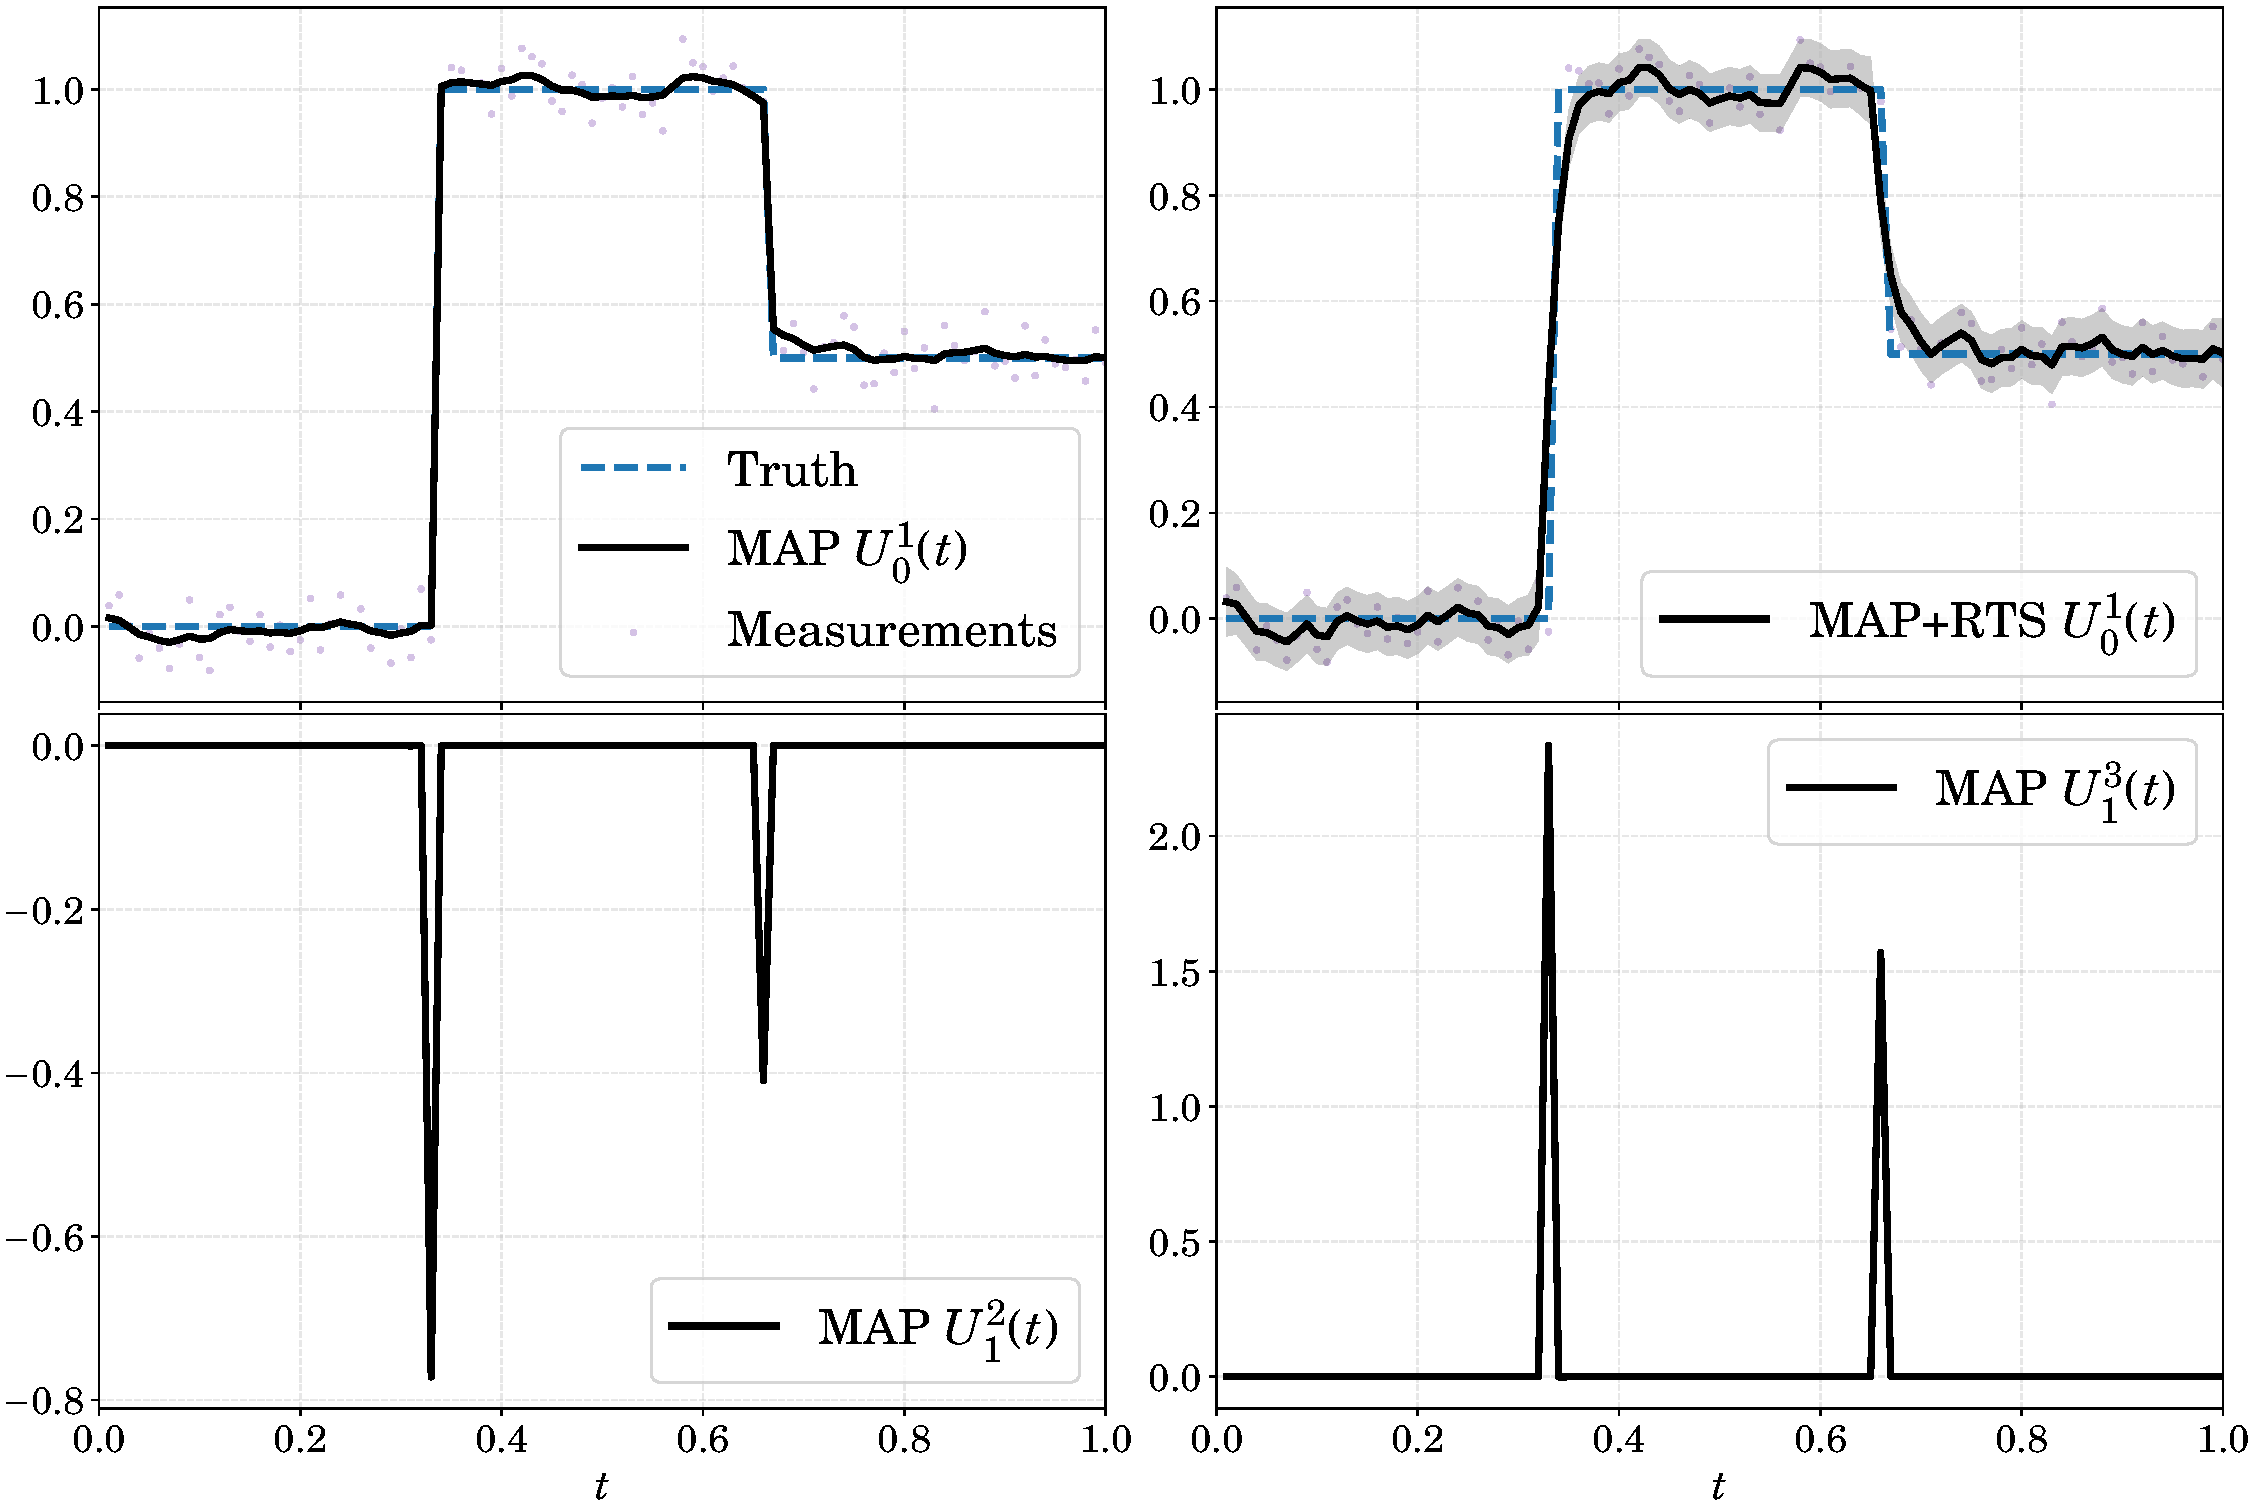
\includegraphics[width=.8\linewidth]{figs/r-ssgp-admm}
	\caption{Regularised SS-DGP regression on a rectangular signal. The uncertainty is quantified by using Equation~\eqref{equ:r-ssdgp-uncertainty} and an RTS smoother.}
	\label{fig:r-ssdgp-admm}
\end{figure}

Another solution is to solve the subproblems of ADMM by using Bayesian solvers instead of deterministic optimisers, resulting in an estimate of the uncertainty in the form of a posterior distribution on the solution. For instance, it is known that the iterated extended Kalman smoother is in some sense equivalent to the Gauss--Newton method~\citep{Bell1994, Simo2020IEKFS}, and \citet{Rui2019ieks} showed that this connection could be extended to the ADMM method. For a review of these, we refer the reader to the discussion in \citet{Rui2020thesis}.

However, if we are only interested in the marginal posterior density $p_{U^1_{0, 1:T} \cond Y_{1:T}}\big(u^1_{0, 1:T} \cond y_{1:T}\big)$ instead of the full density $p_{V_{1:T} \cond Y_{1:T}}(v_{1:T} \cond y_{1:T})$, then we can leverage the hierarchical nature of DGPs to approximate the marginal density efficiently. In order to do so, we can write the approximation
\begin{equation}
	\begin{split}
		&p_{U^1_{0, 1:T} \cond U^2_{1, 1:T}, U^3_{1, 1:T}, Y_{1:T}}\big(u^1_{0, 1:T} \cond u^2_{1, 1:T}, u^3_{1, 1:T}, y_{1:T}\big) \\
		&\approx p_{U^{1}_{0, 1:T} \cond Y_{1:T}}\big(u^1_{0, 1:T} \cond u^{2, \star}_{1, 1:T}, u^{3, \star}_{1, 1:T}, y_{1:T}\big),
		\label{equ:r-ssdgp-uncertainty}
	\end{split}
\end{equation}
where $u^{2, \star}_{1, 1:T}, u^{3, \star}_{1, 1:T}$ stand for the MAP estimates of $U^{2}_{1, 1:T}\mid y_{1:T}$ and $U^{3}_{1, 1:T} \mid y_{1:T}$. Afterwards, computing $p_{U^1_{0, 1:T} \cond Y_{1:T}}\big(u^1_{0, 1:T} \cond y_{1:T}\big)$ simply consists in solving a standard GP regression problem, which can be obtained in closed form~\citep{Zhao2021RSSGP}.

Figure~\ref{fig:r-ssdgp-admm} illustrates such an example of regularised SS-DGP, where we set the sparsity inducing matrices to be identity matrices~\citep{Zhao2021RSSGP}. The latent states $U^2_1$ and $U^3_1$ exhibit spiking behaviours, being almost zero except at the two discontinuities.
